\section{Computationally Expensive Acquisition Functions}
%-----------------------------------------------------------------------
\begin{frame}[c]{Computationally Expensive Acquisition Functions}
%\framesubtitle{Knowledge Gradient - Concept}
\framesubtitle{One-Step Look Ahead}

\begin{figure}
  \centering
  \begin{tikzpicture}
    \node<+> (img1) {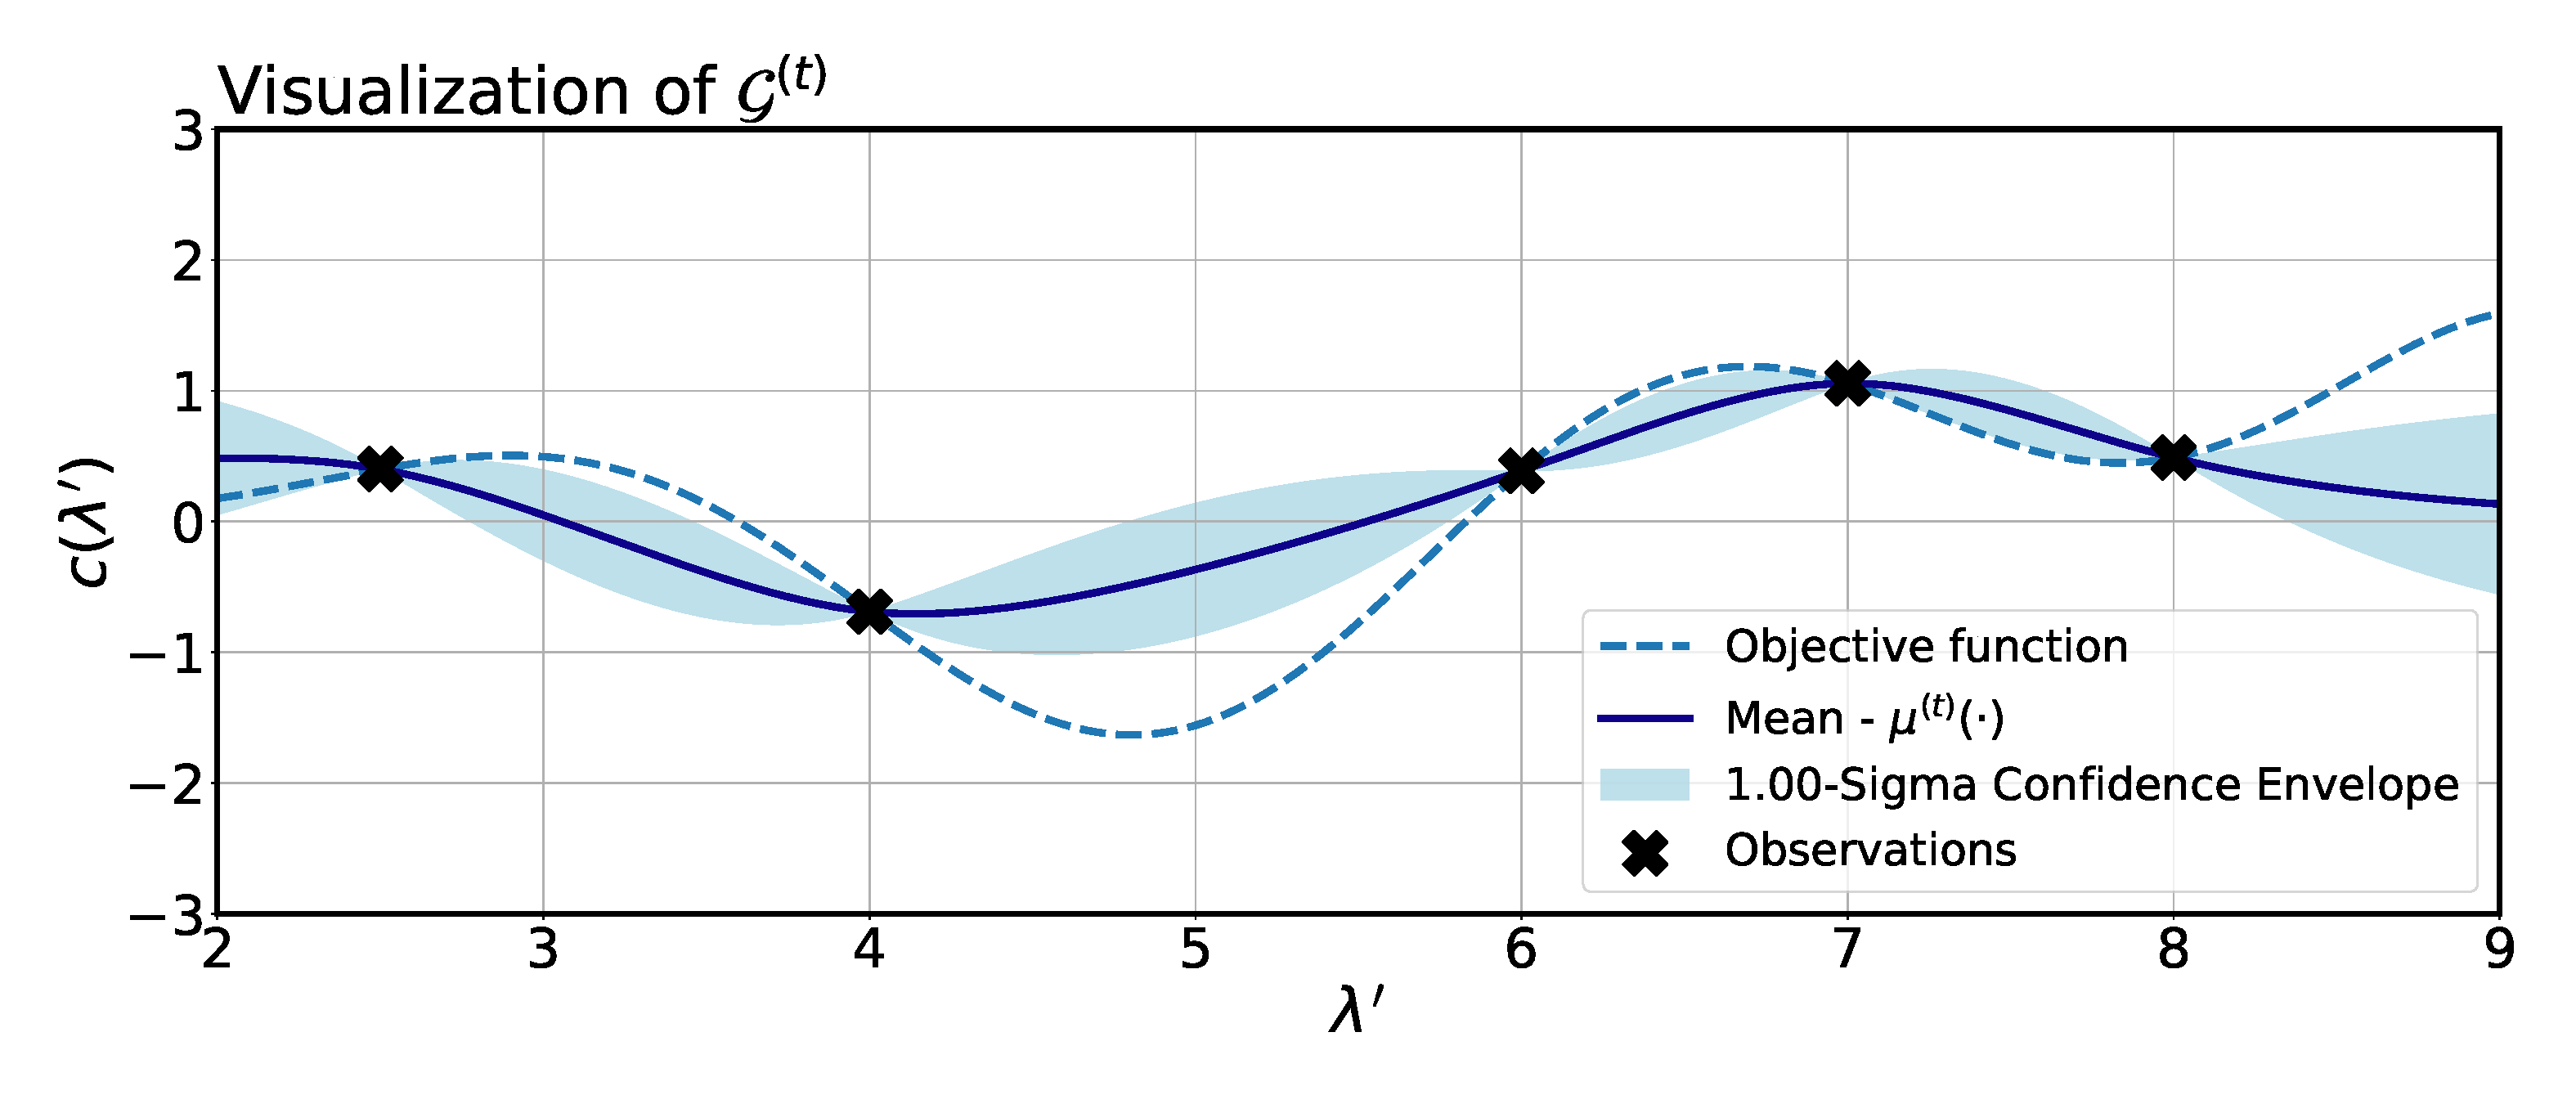
\includegraphics[width=\textwidth, height=0.7\textheight, keepaspectratio=true]{images/acq_func_images/kg/look_ahead_1.pdf}};
    \node<.> [below=0.01\belowcaptionskip of img1, align=center]{Once more, assume such a surrogate GP $\iter{\gp}(\cdot)$ at time-step $\bocount$.};

    \node<+> (img2) {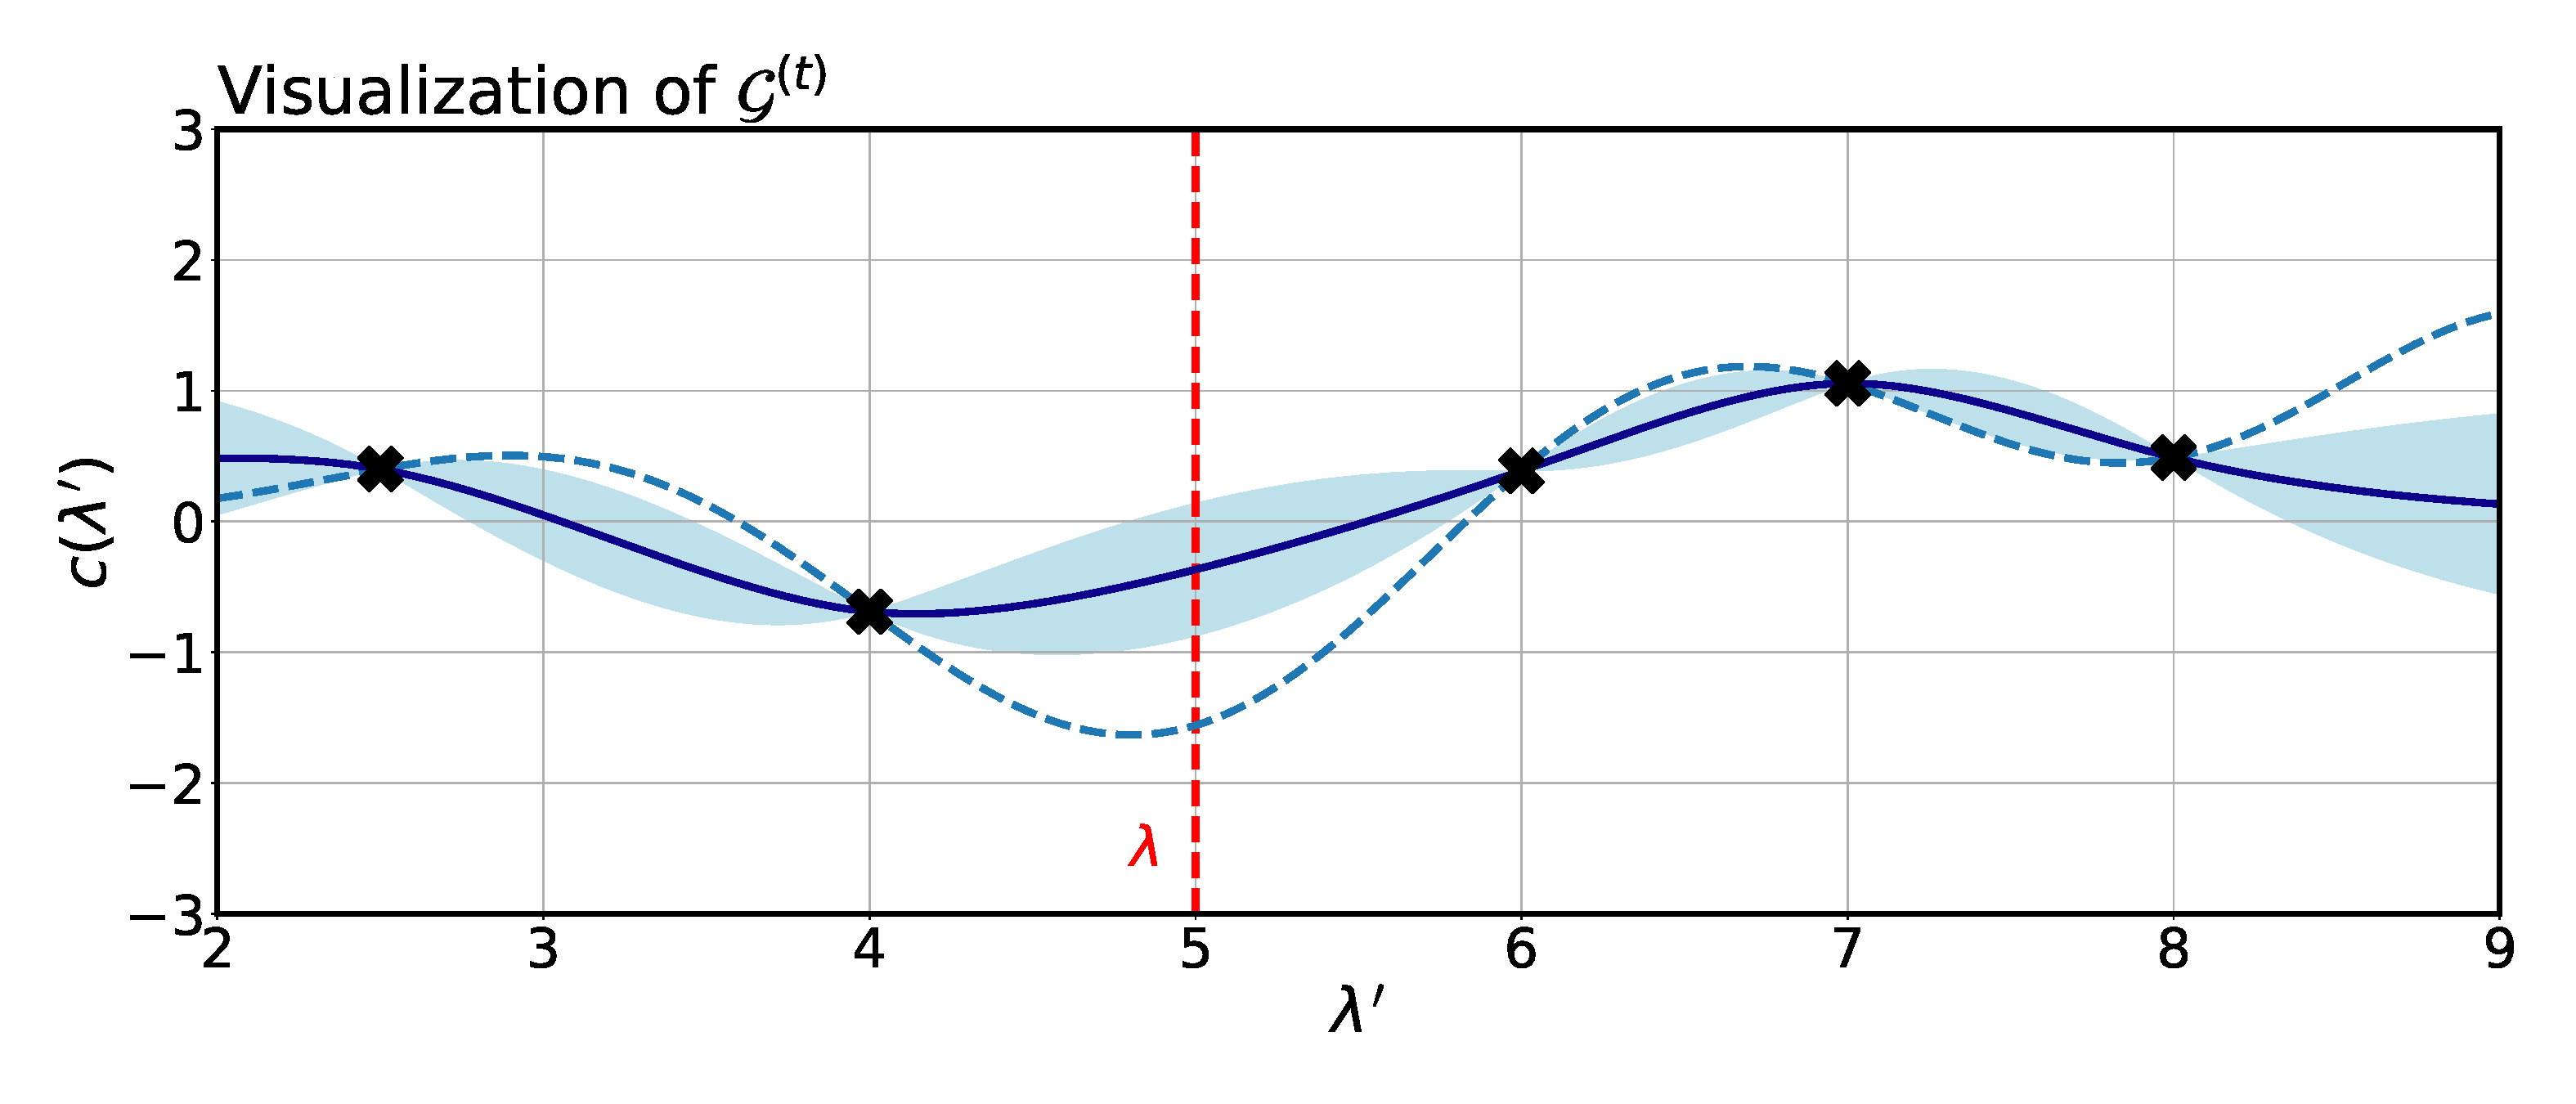
\includegraphics[width=\textwidth, height=0.7\textheight, keepaspectratio=true]{images/acq_func_images/kg/look_ahead_1a.pdf}};
    \node<.> [below=0.01\belowcaptionskip of img2, align=center]{Imagine that we sample at a random configuration $\conf$};

    \node<+> (img3) {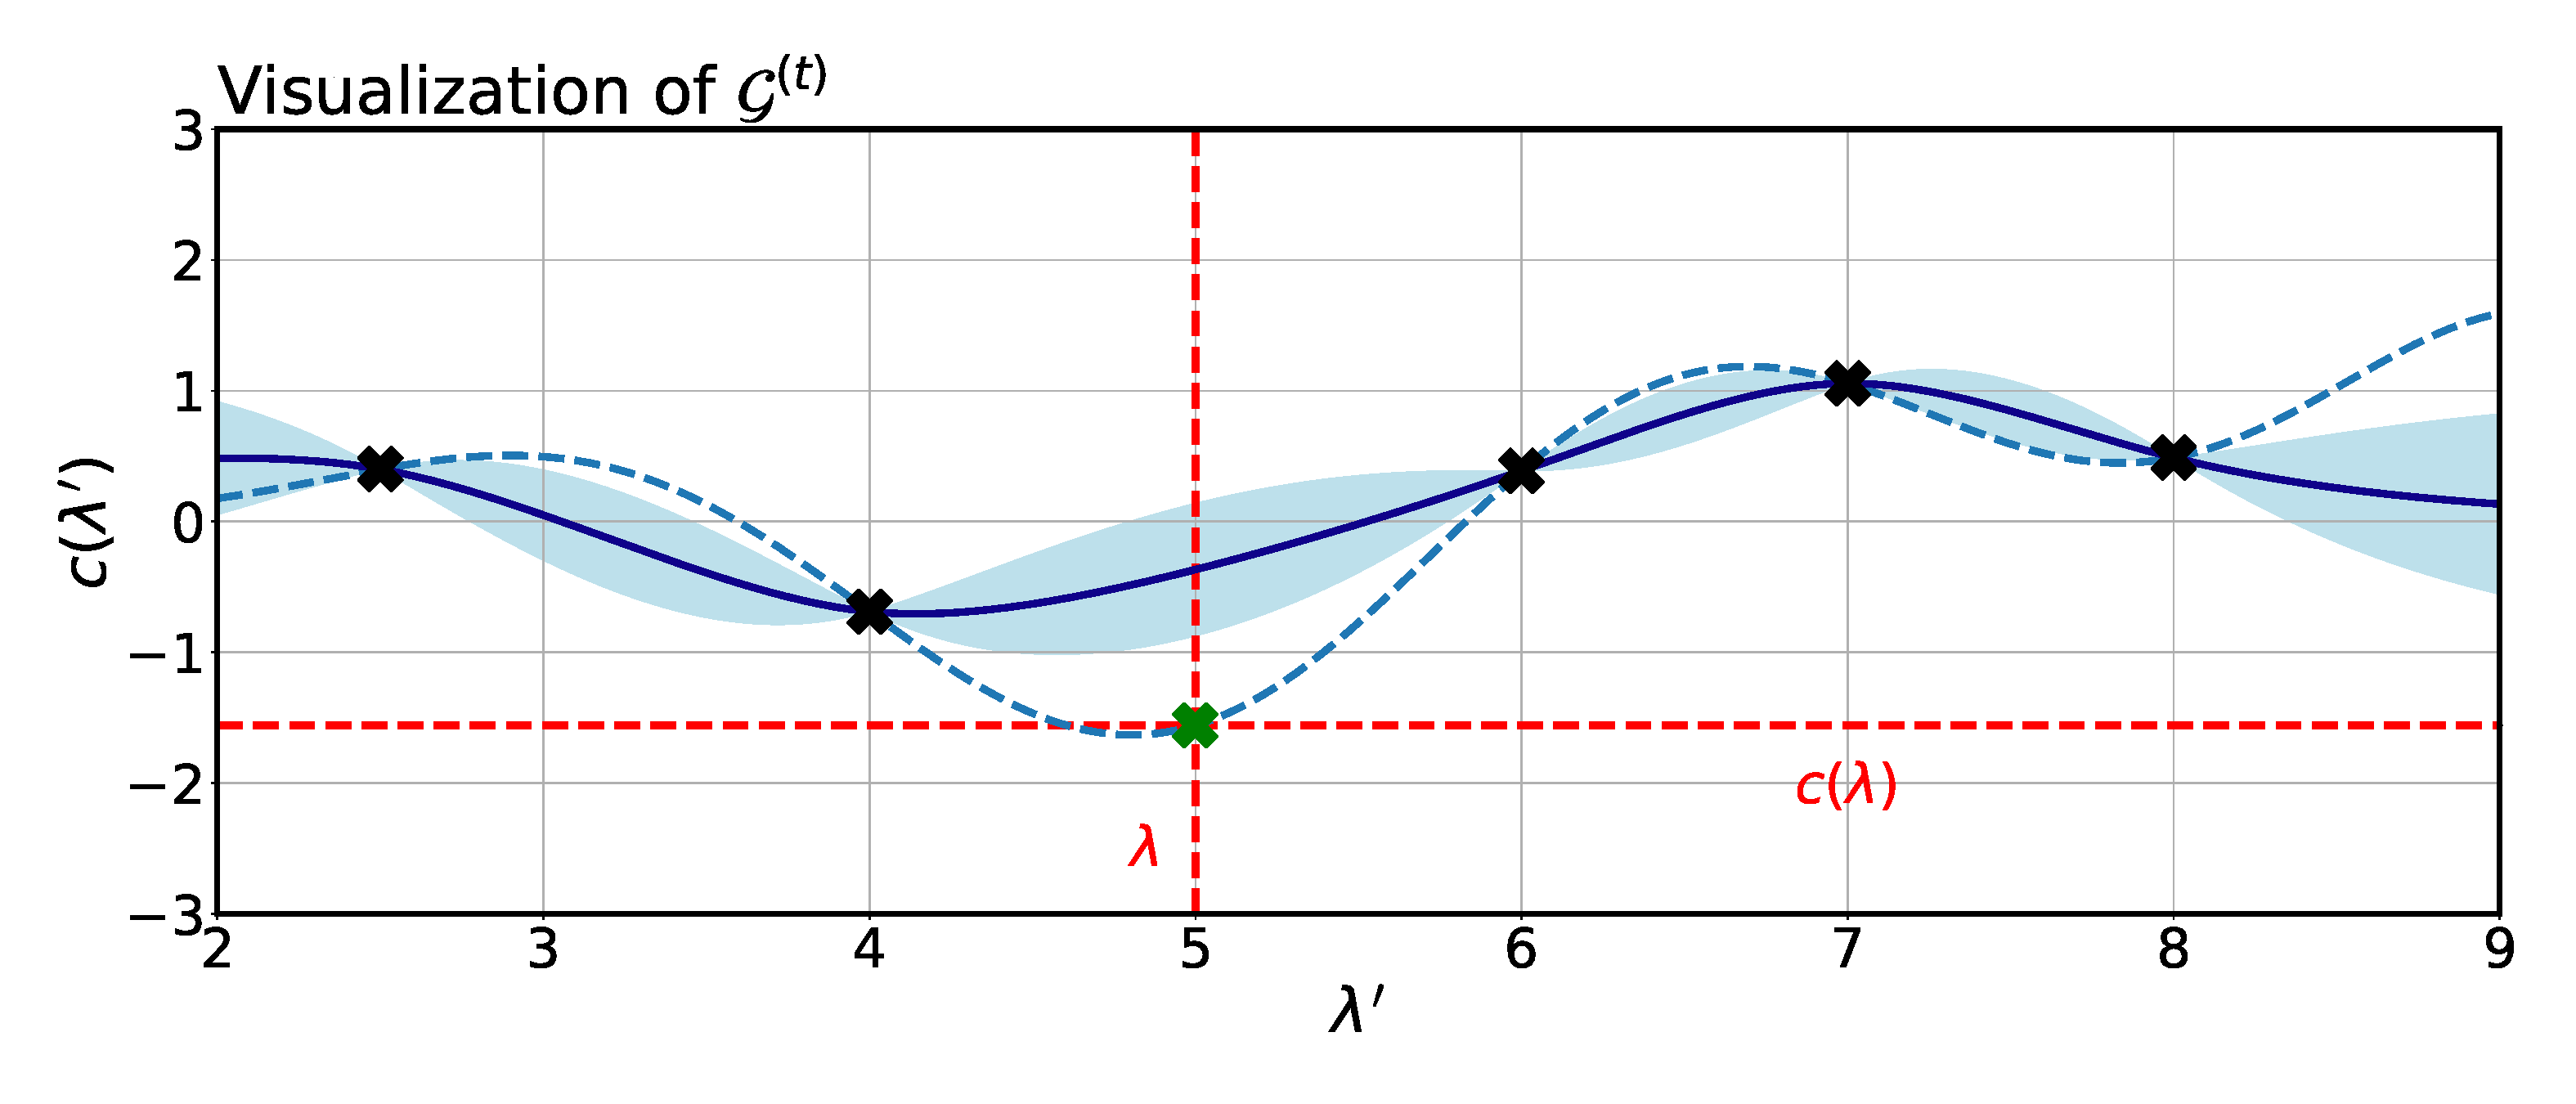
\includegraphics[width=\textwidth, height=0.7\textheight, keepaspectratio=true]{images/acq_func_images/kg/look_ahead_1b.pdf}};
    \node<.> [below=0.01\belowcaptionskip of img3, align=center]{We would then observe the cost $\cost(\conf)$ at this imaginary configuration $\conf$};
    
    \node<+> (img4) {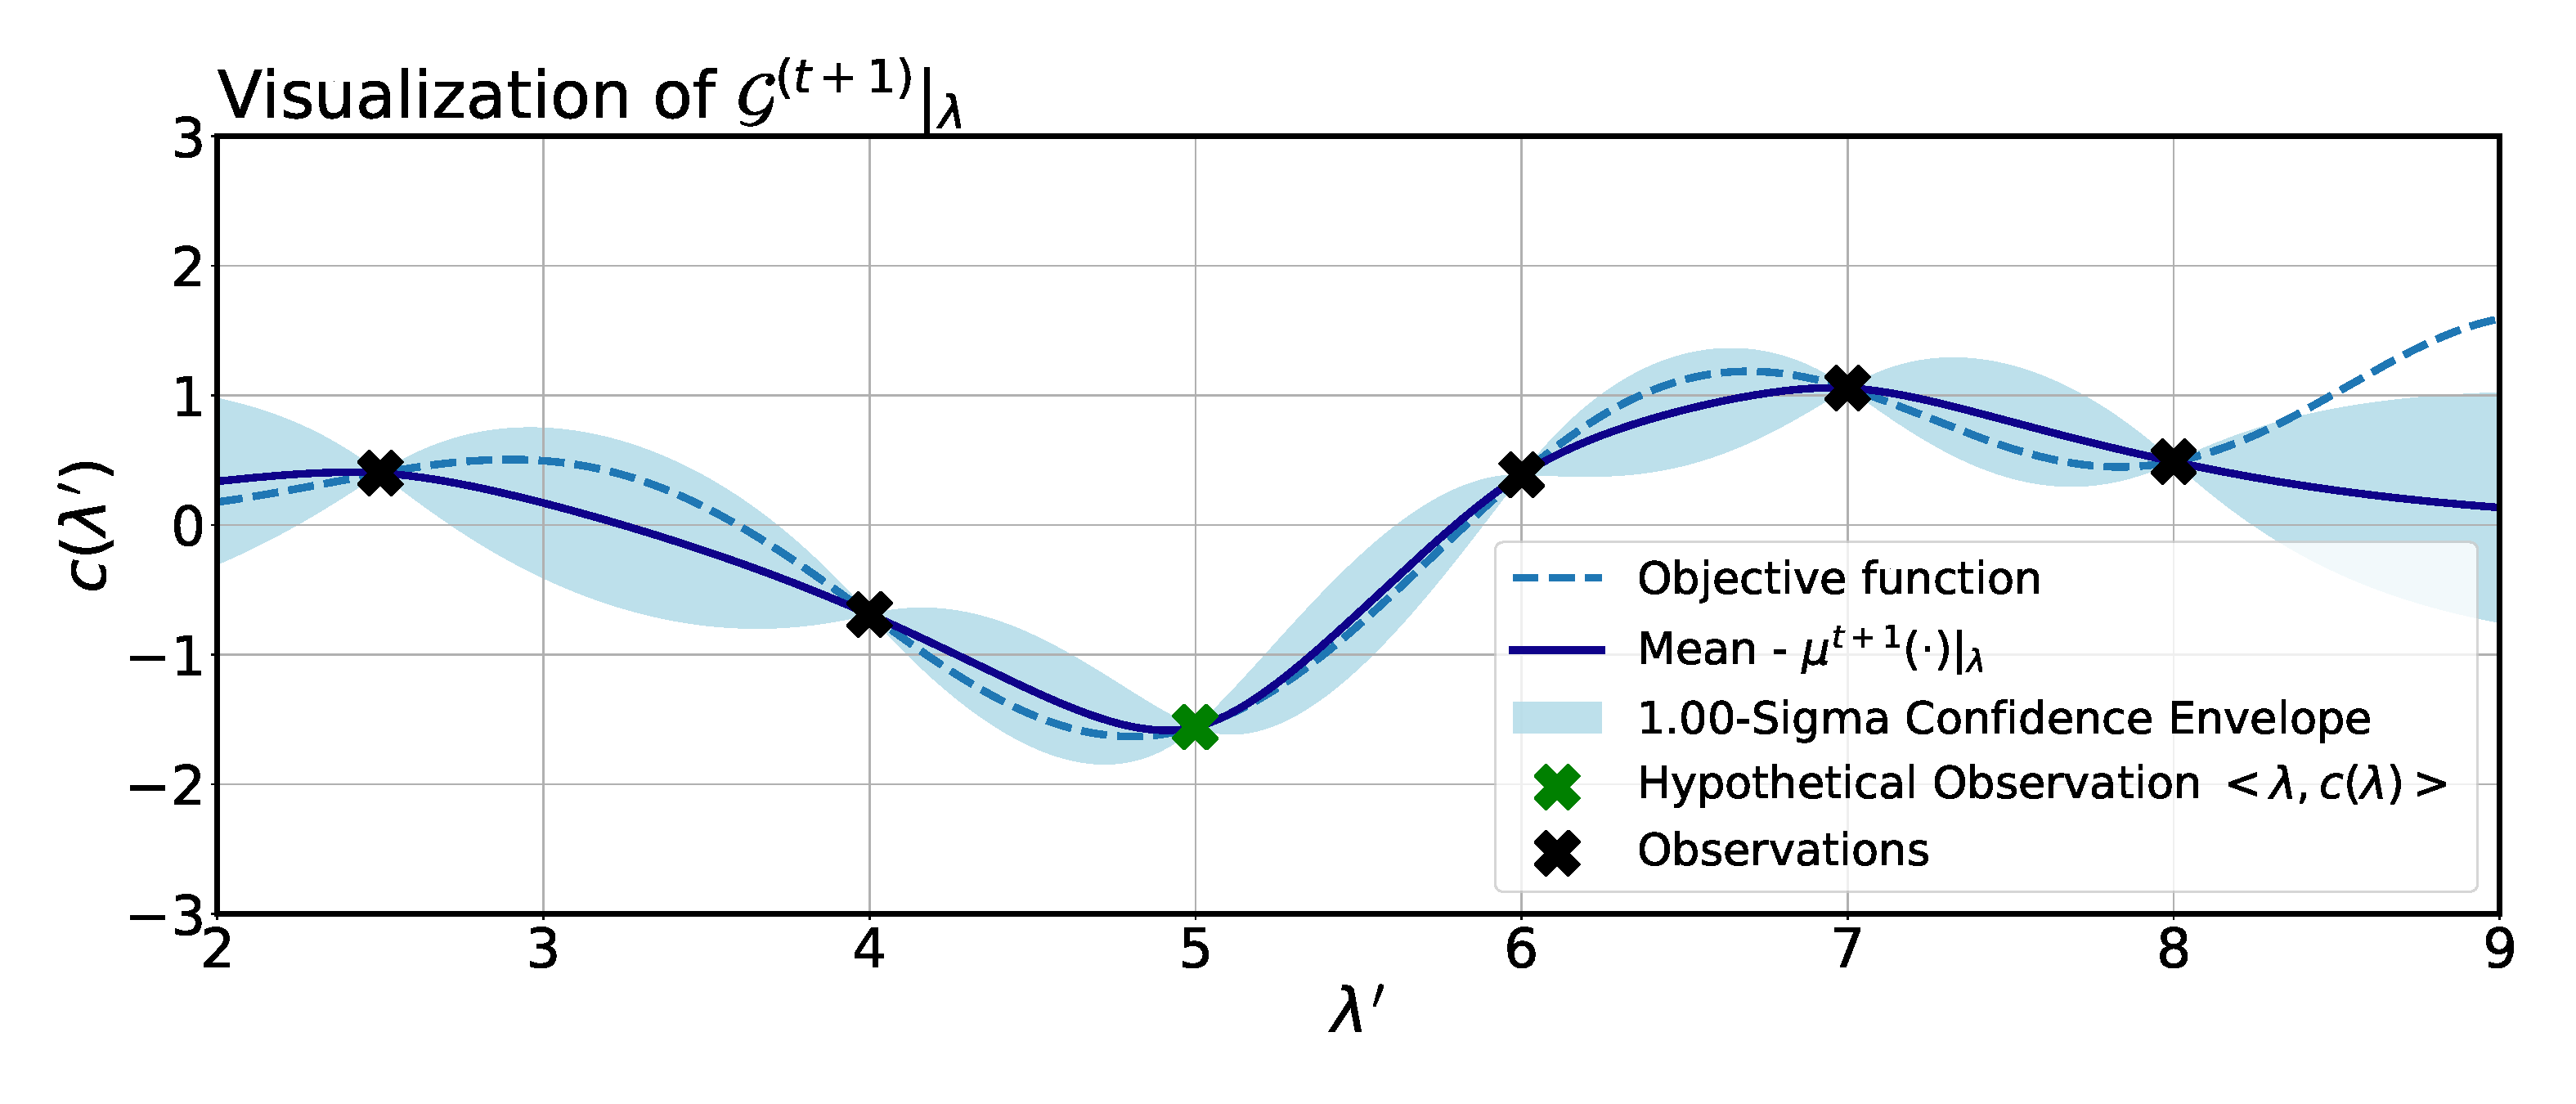
\includegraphics[width=\textwidth, height=0.7\textheight, keepaspectratio=true]{images/acq_func_images/kg/look_ahead_3.pdf}};
    \node<.> [below=0.01\belowcaptionskip of img4, align=center]{Then, $\iter[\bocount+1]{\gp}(\cdot\given {\conf})$ \emph{might} look like this. This is called a "1-step look ahead".};
    
    \node<+> (img5) {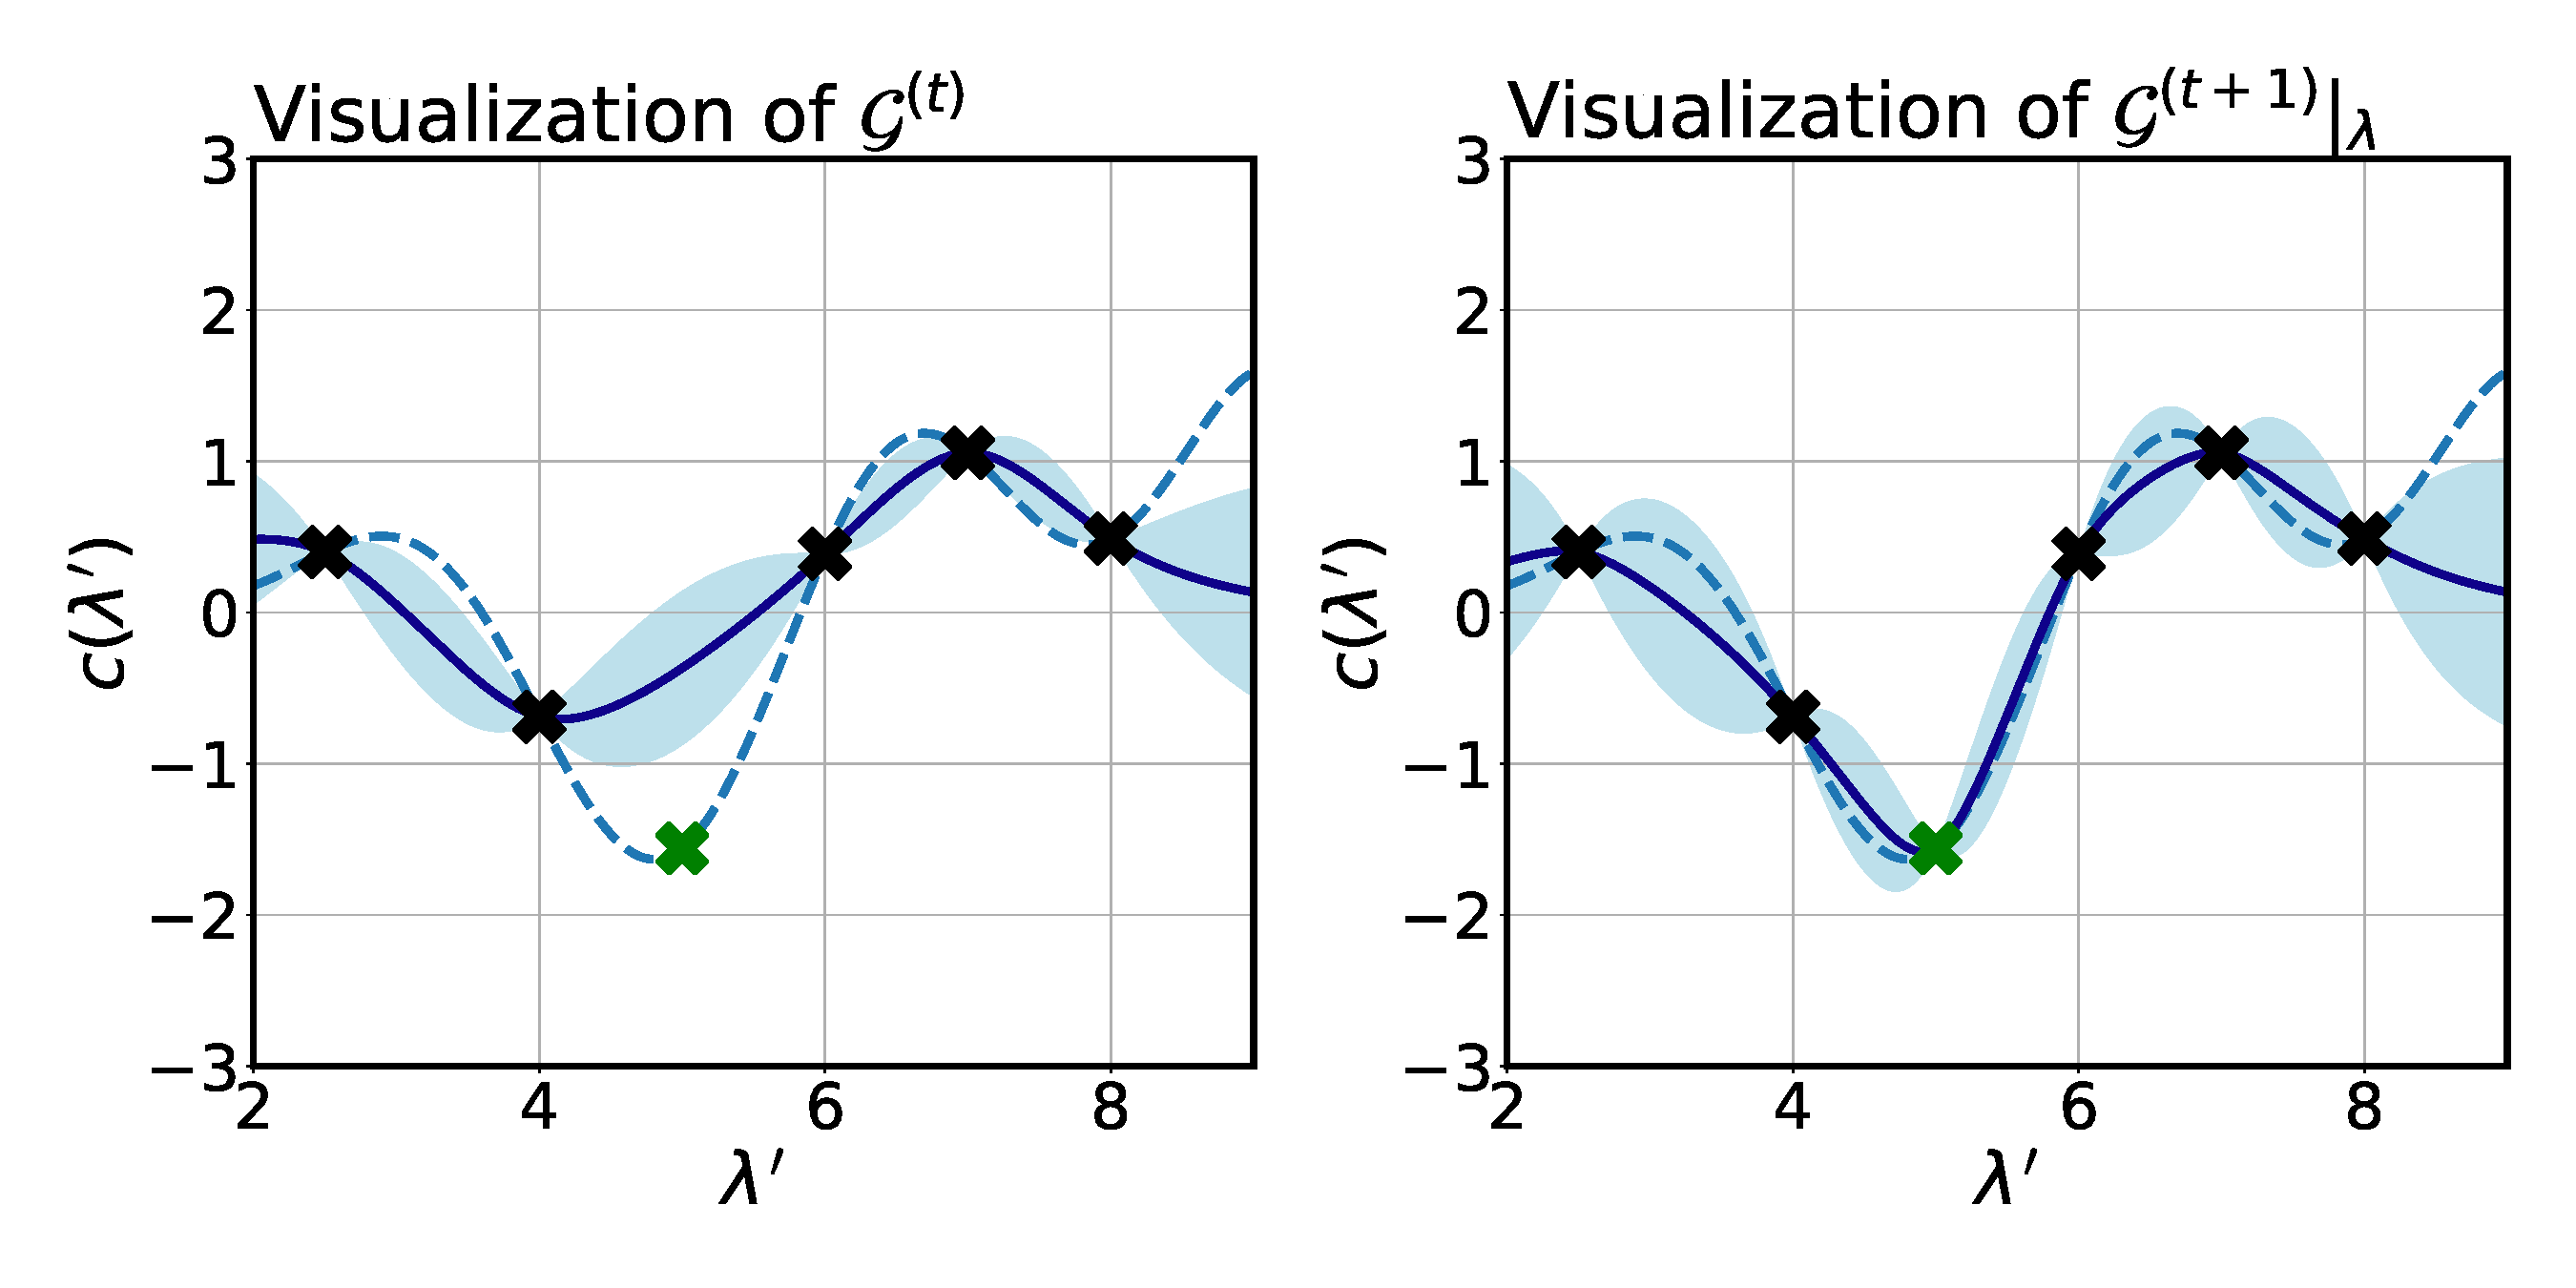
\includegraphics[width=\textwidth, height=0.7\textheight, keepaspectratio=true]{images/acq_func_images/kg/look_ahead_3a.pdf}};
    \node<.> [below=0.01\belowcaptionskip of img5, align=center]{A comparison of $\iter{\gp}(\cdot)$ and $\iter[\bocount+1]{\gp}(\cdot\given {\conf})$ for a given $\conf$.};
    
    \node<+> (img6) {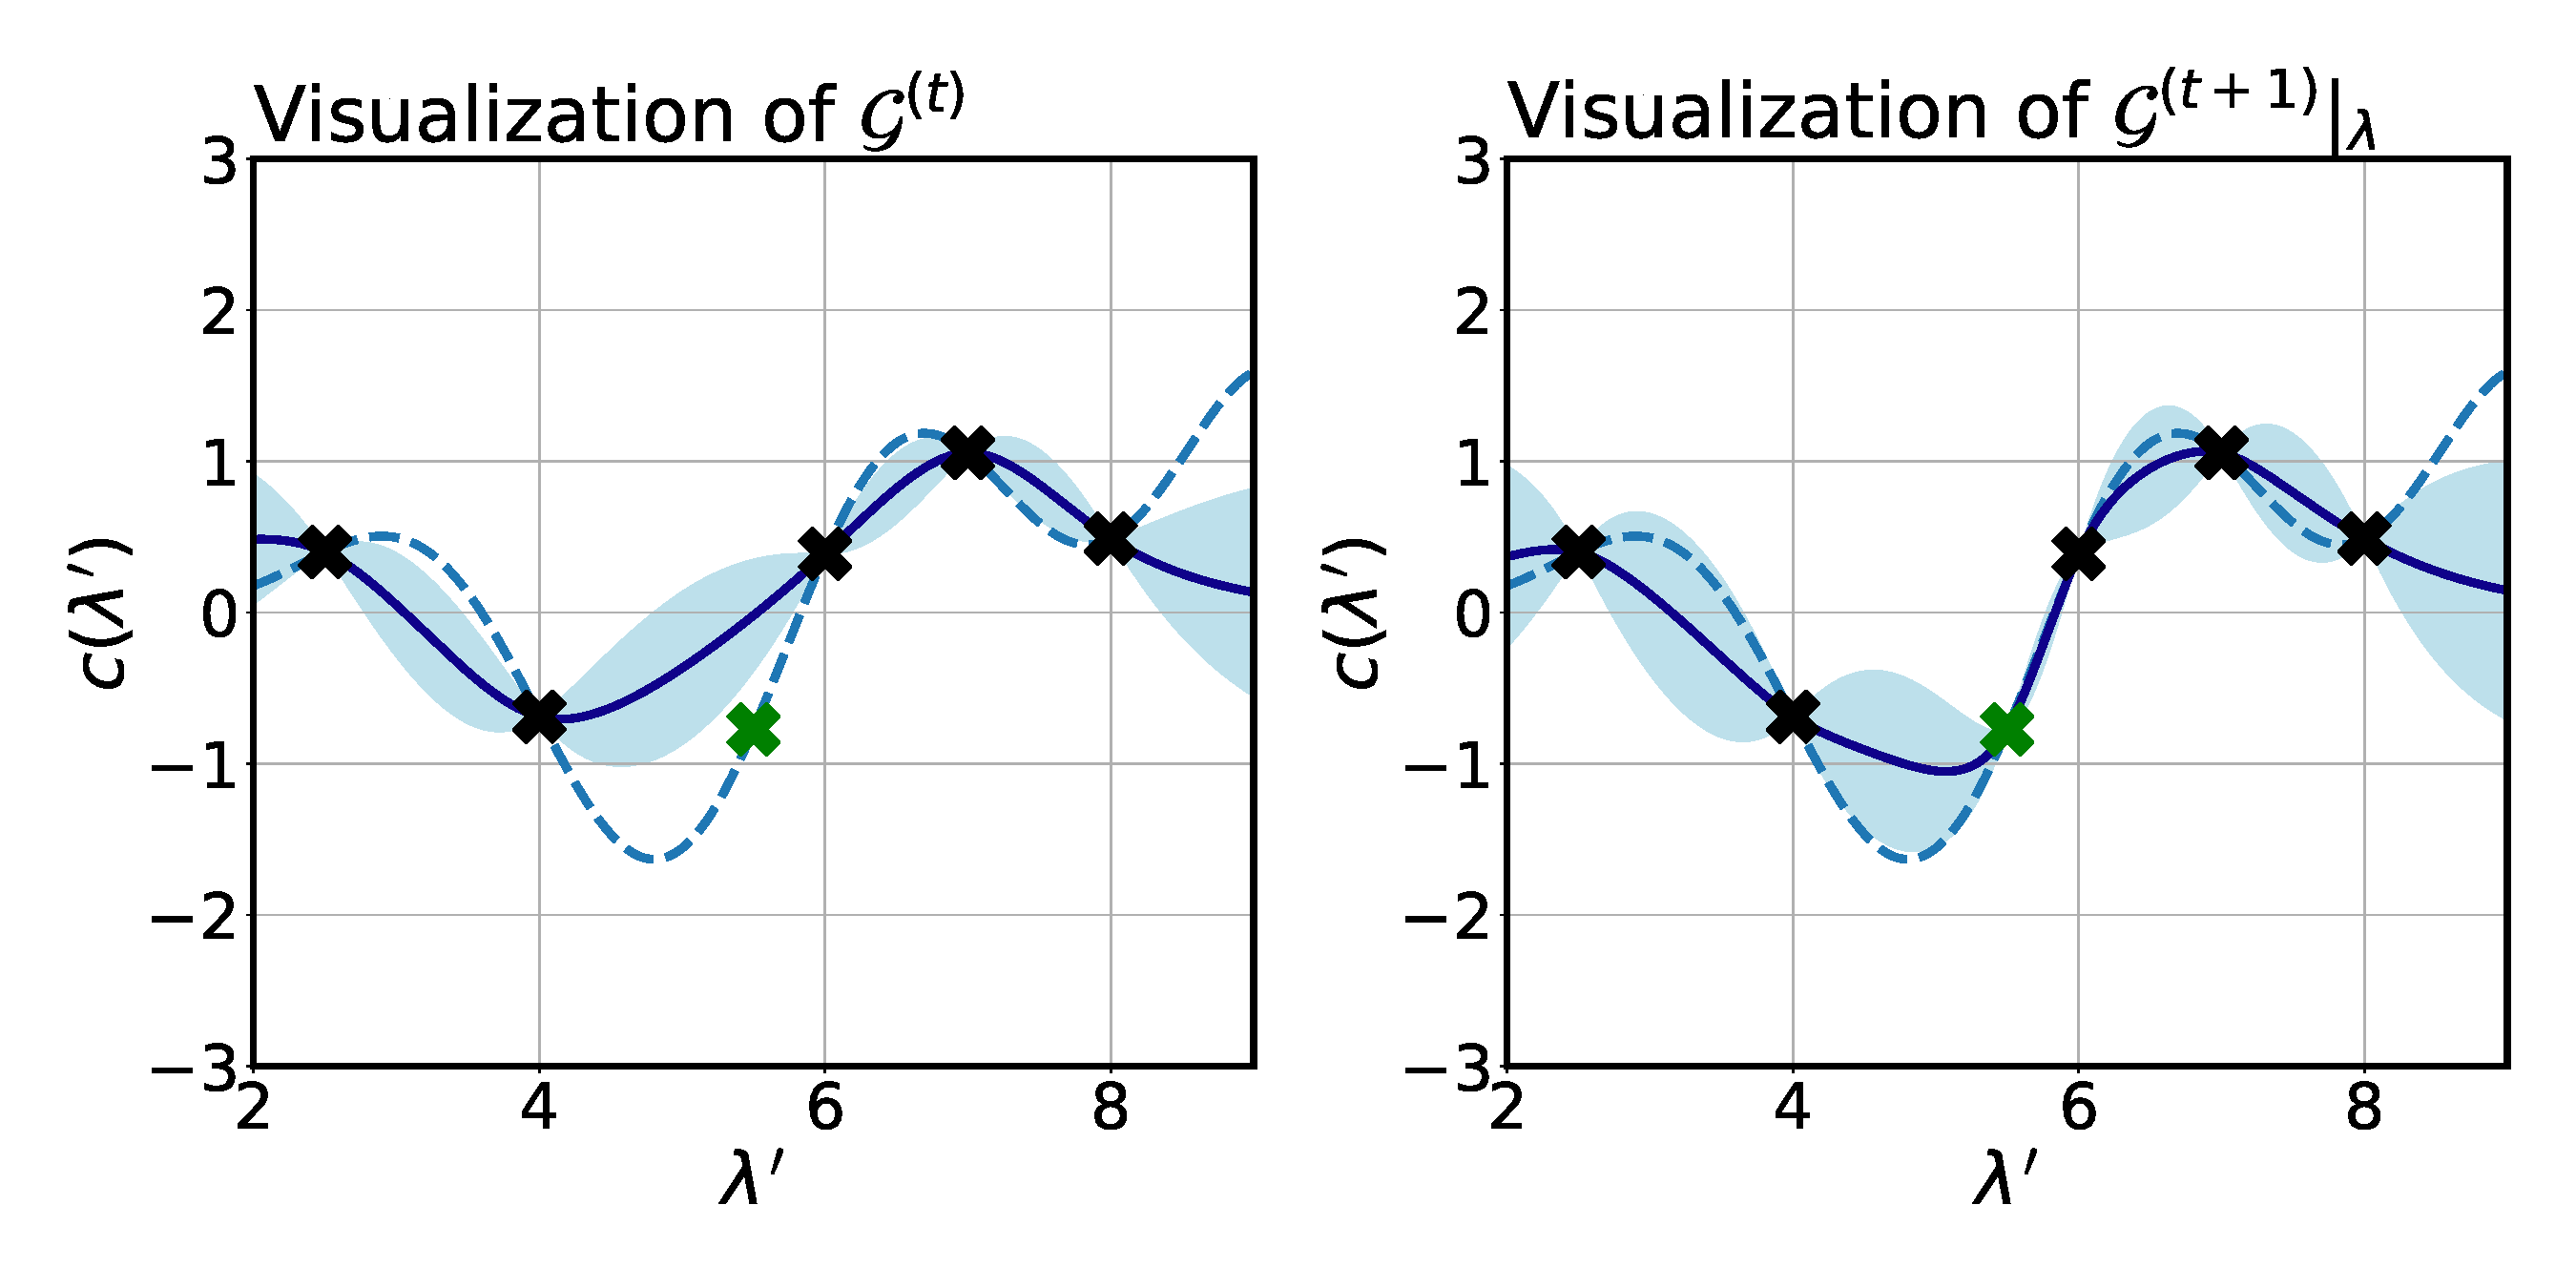
\includegraphics[width=\textwidth, height=0.7\textheight, keepaspectratio=true]{images/acq_func_images/kg/look_ahead_3b.pdf}};
    \node<.> [below=0.01\belowcaptionskip of img6, align=center]{A comparison of $\iter{\gp}(\cdot)$ and $\iter[\bocount+1]{\gp}(\cdot\given {\conf})$ for a different $\conf$.};
    
    \node<+> (img7) {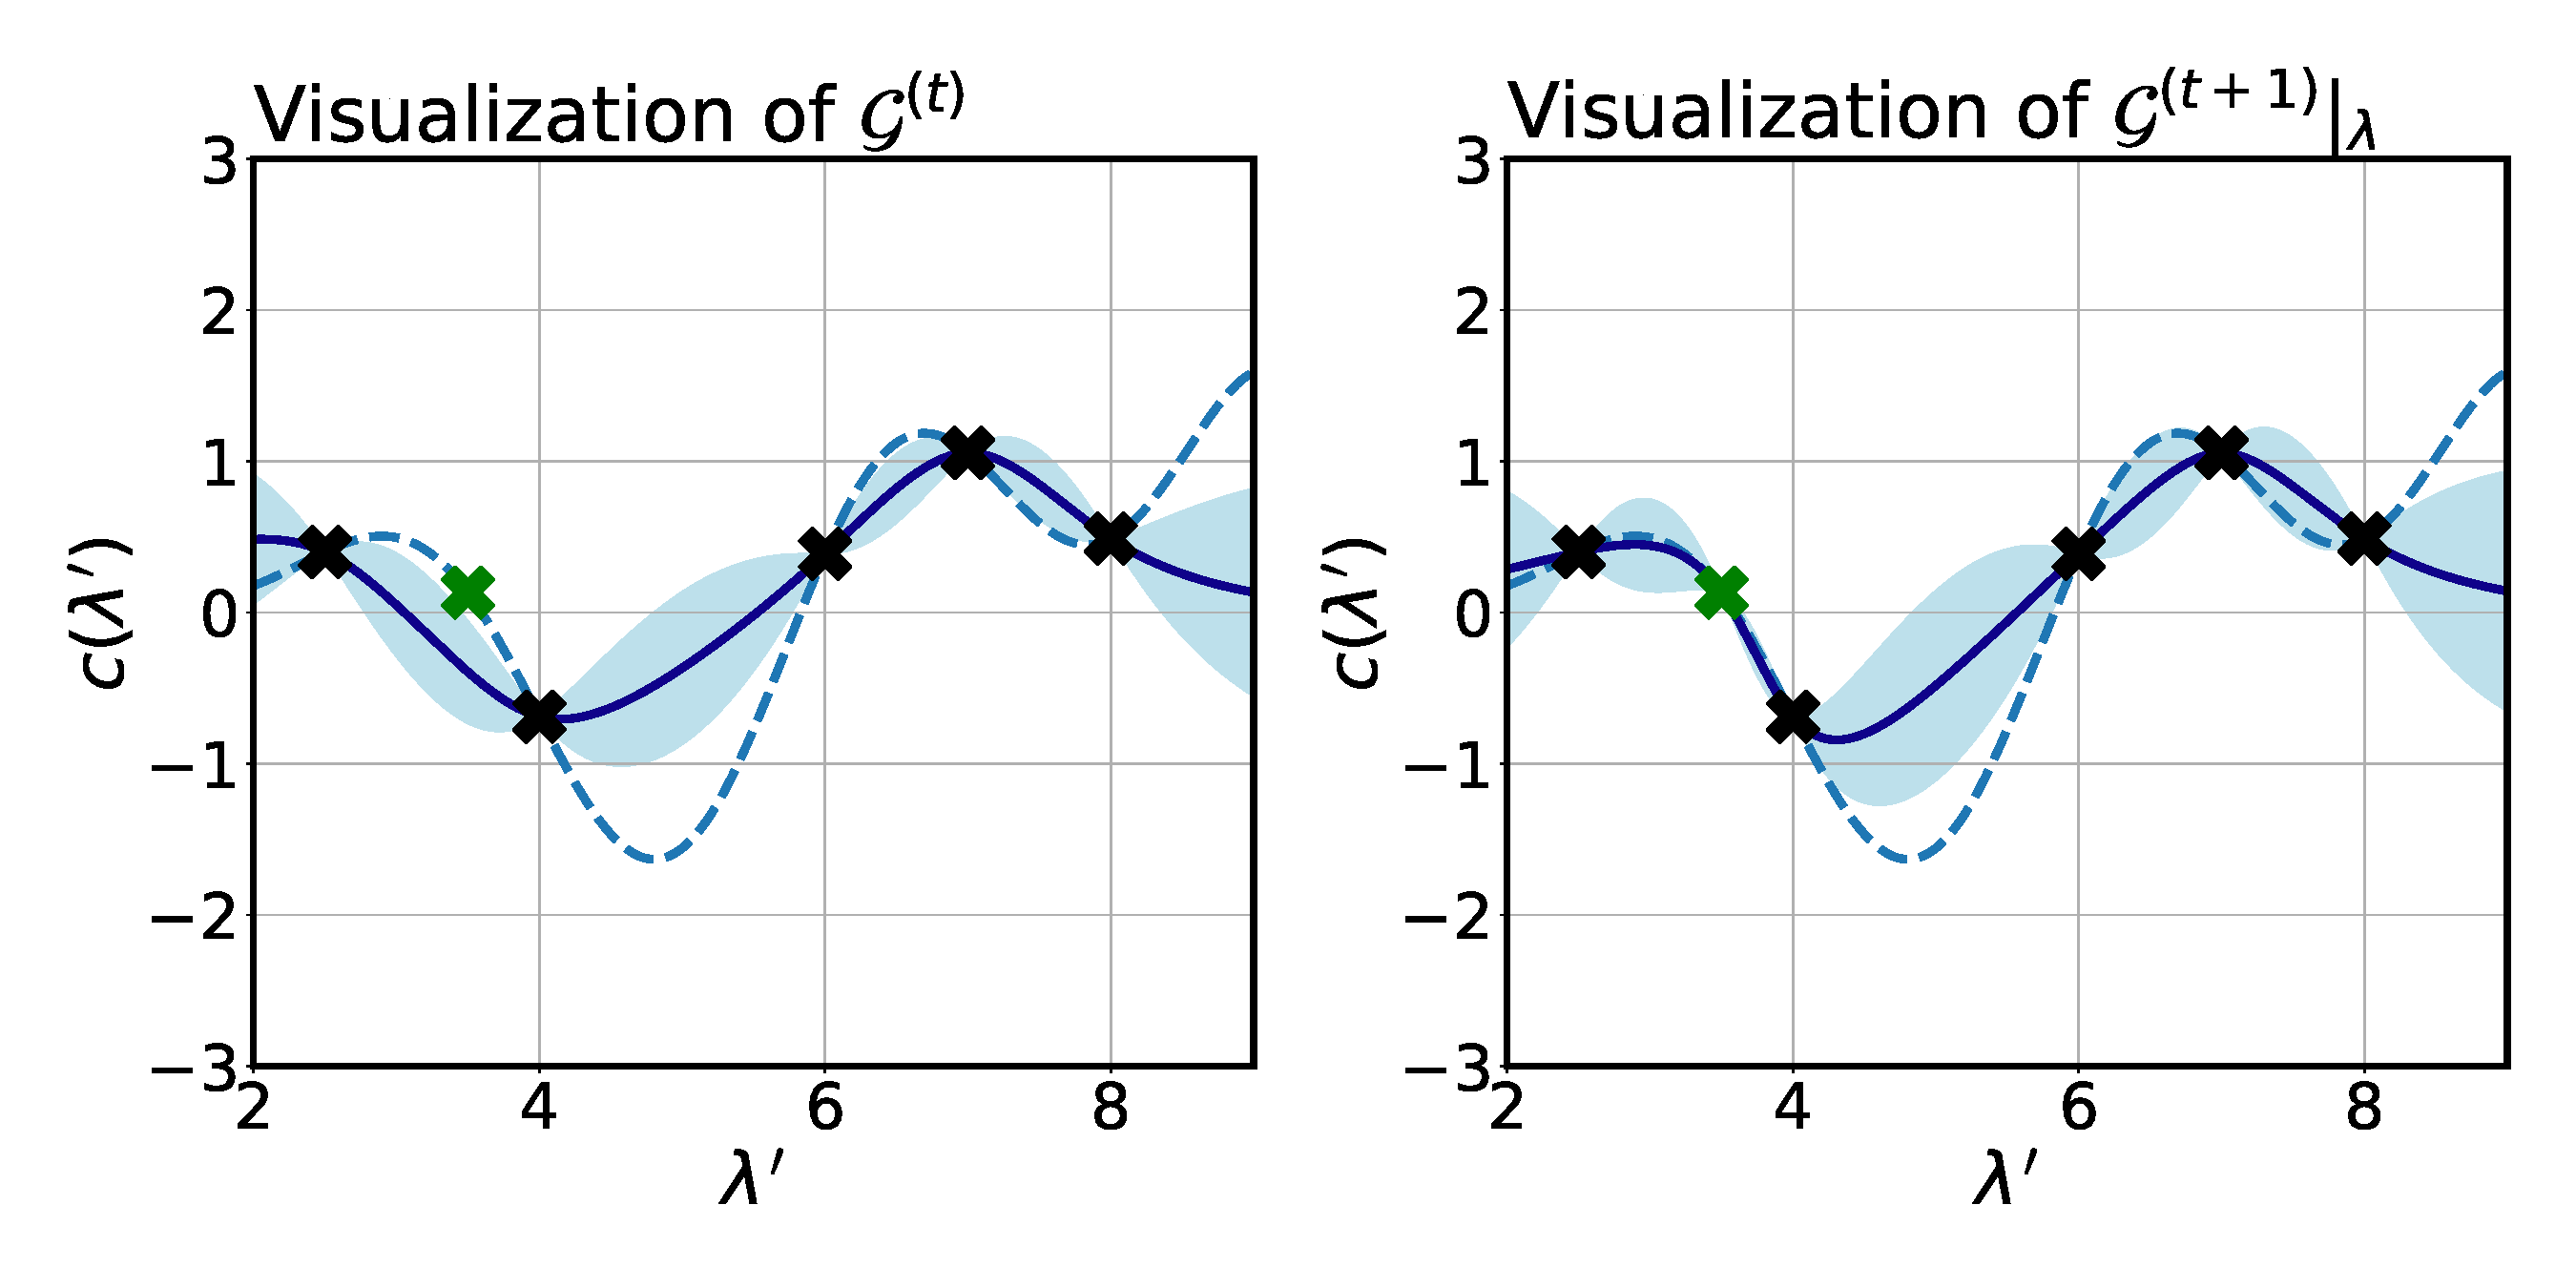
\includegraphics[width=\textwidth, height=0.7\textheight, keepaspectratio=true]{images/acq_func_images/kg/look_ahead_3c.pdf}};
    \node<.> [below=0.01\belowcaptionskip of img7, align=center]{A comparison of $\iter{\gp}(\cdot)$ and $\iter[\bocount+1]{\gp}(\cdot\given {\conf})$ for yet another $\conf$};

\comment{Pardon the inconsistent label for the vertical red line - it's a bug that would need some time to trace and solve, but should not affect the readability of the plots.}

\comment{Here we are fantasizing how the GP would look like if we had done an actual evaluation at the chosen configuration, i.e. had observed the actual cost incurred for using that configuration.}

\comment{Mean - $\iter[\bocount+1]{\mean} \given_{\conf}$, Variance - $\iter[\bocount+1]{\left(\variance\right)} \given_{\conf}$, Minimum of the mean function - $\iter[\bocount+1]{\left(\mean^*\right)} \given_{\conf}$. It should be noted that all these quantities are now conditionally dependent on our choice of $\conf$, as demonstrated by the | sign next to all these quantities.}

\comment{This distribution is purely hypothetical - as shown by the conditional - and is called a one-step look-ahead. Just a re-statement of the GP's conditional nature at $\bocount+1$. Since we don't actually have the underlying objective function available in real-life scenarios, it is impossible to generate the true look-ahead without actually performing an evaluation.}
  \end{tikzpicture}
\end{figure}
\end{frame}
%-----------------------------------------------------------------------

\begin{frame}[c]{Computationally Expensive Acquisition Functions - KG}
\framesubtitle{Knowledge Gradient - Concept}

\begin{figure}
  \centering
  \begin{tikzpicture}
    \node<+> (img1) {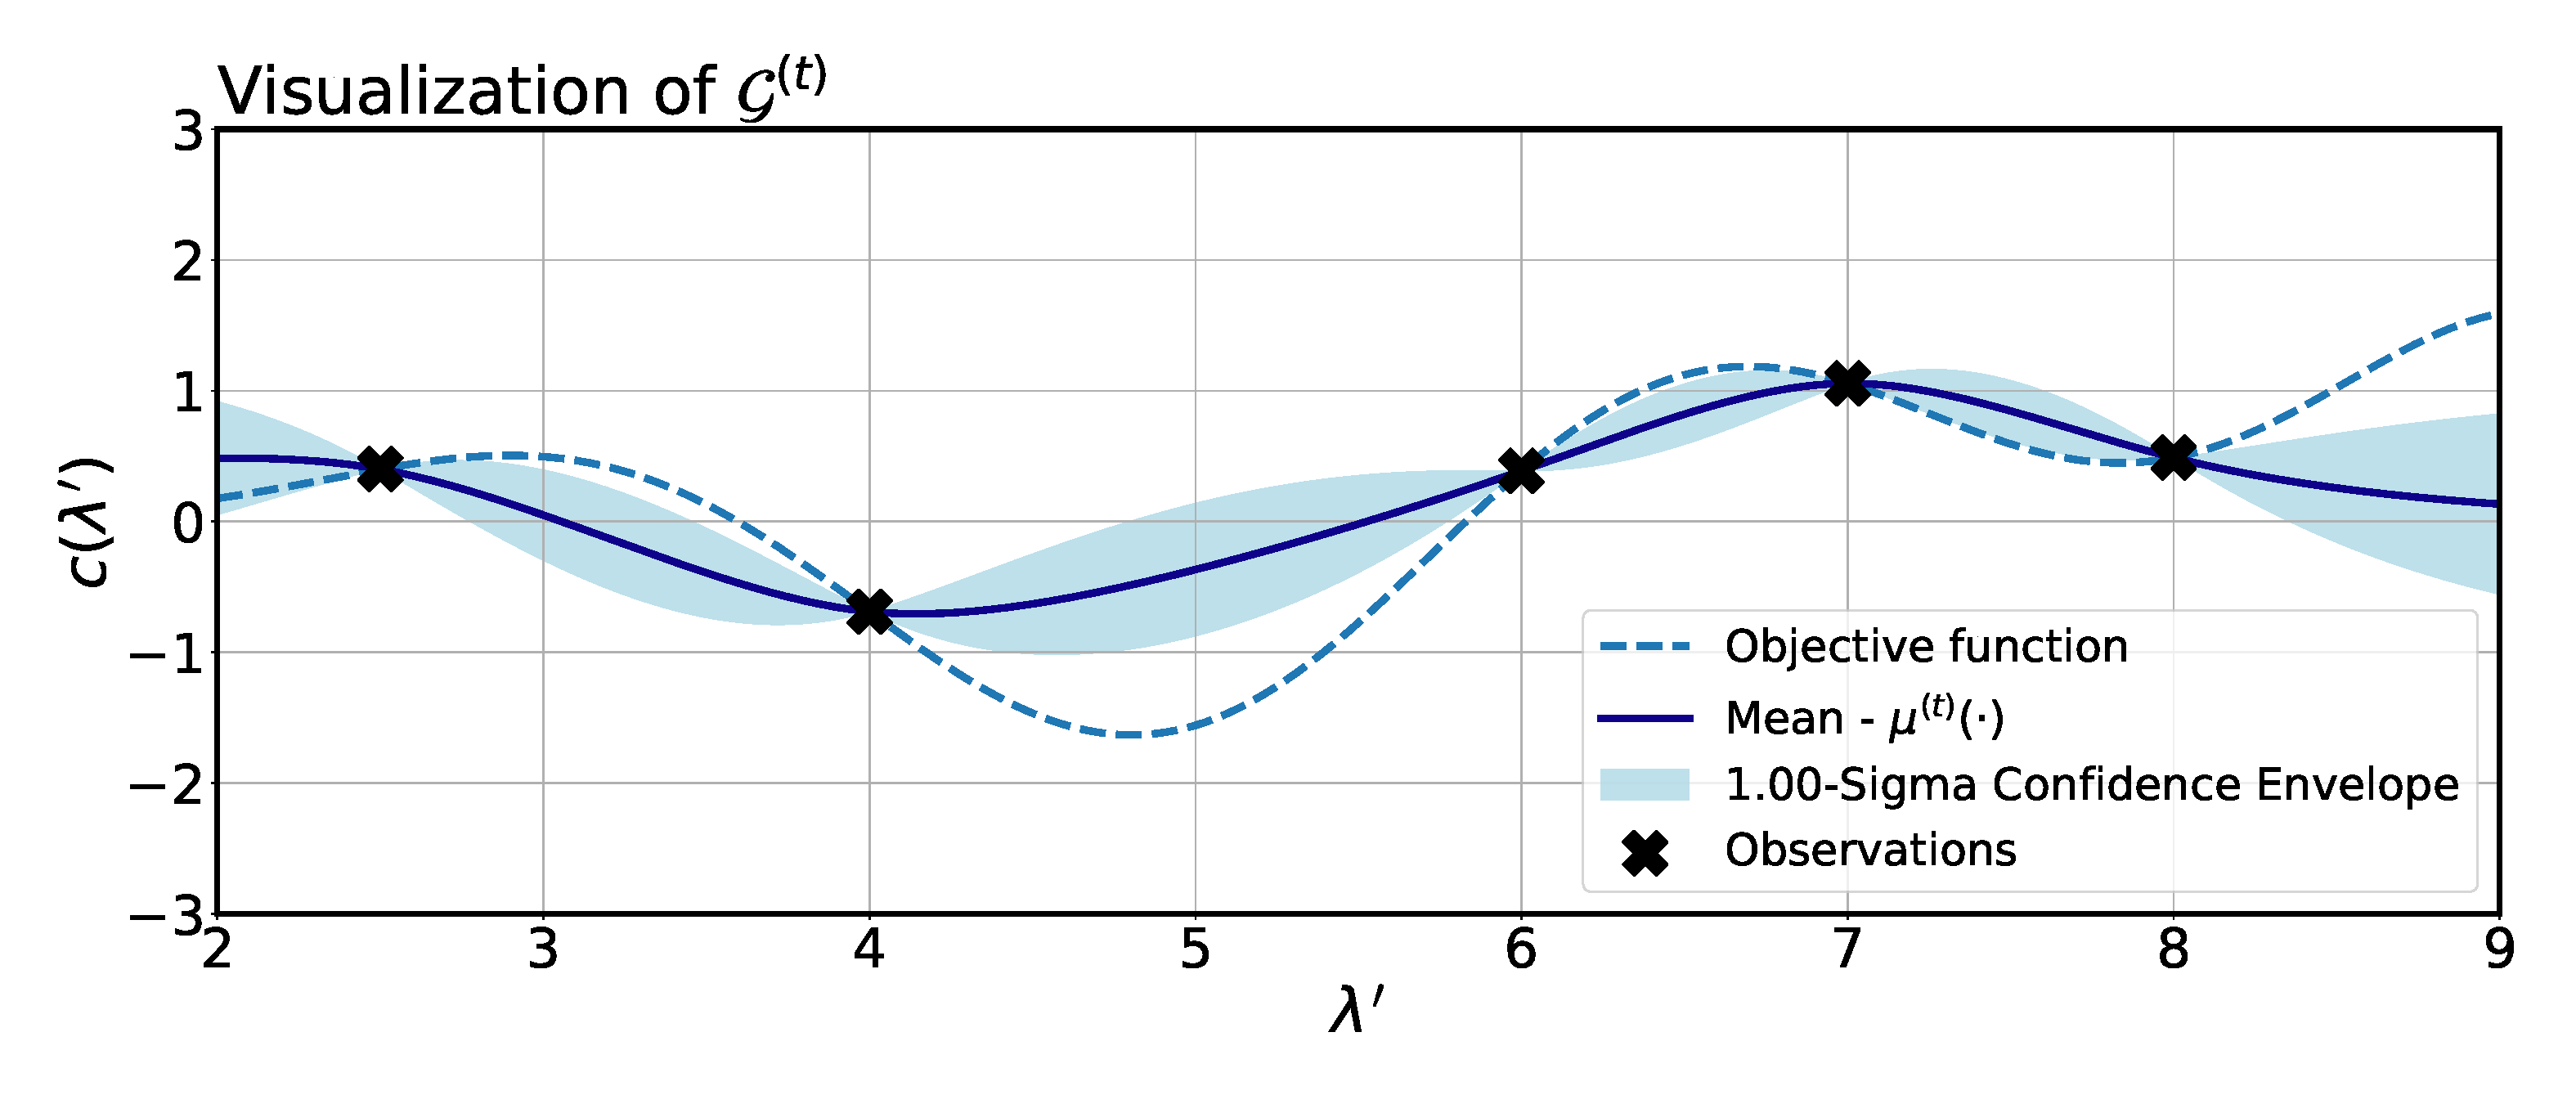
\includegraphics[width=\textwidth, height=0.7\textheight, keepaspectratio=true]{images/acq_func_images/kg/look_ahead_1.pdf}};
    \node<.> [below=0.01\belowcaptionskip of img1, align=center]{Once more, assume such a surrogate function GP $\iter{\gp}(\cdot)$ at time-step $\bocount$.};
    
    \node<+> (img2) {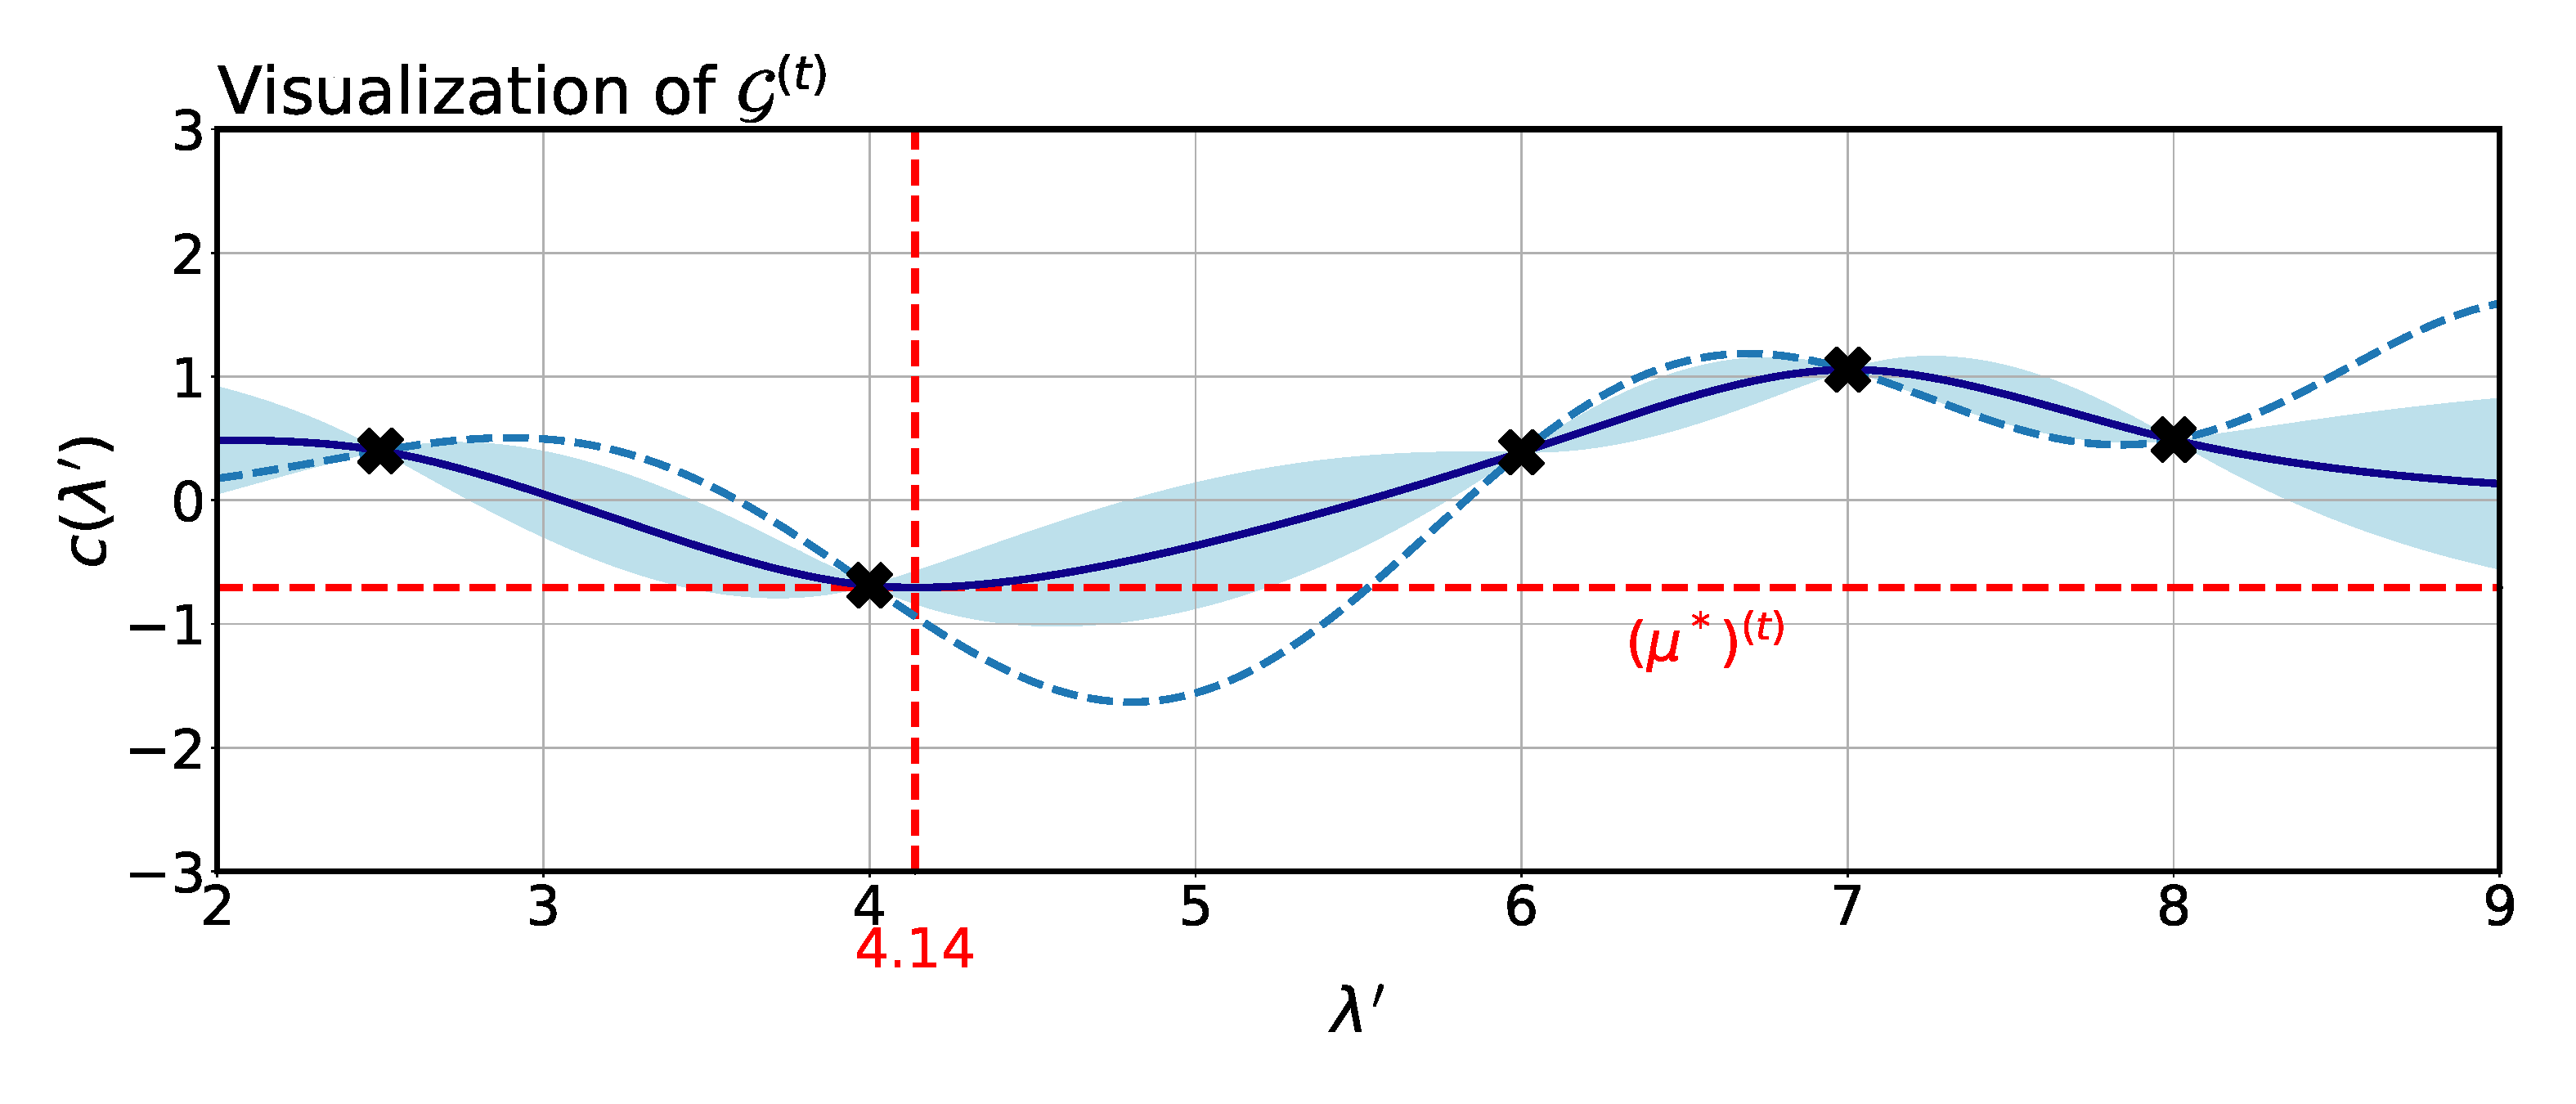
\includegraphics[width=\textwidth, height=0.7\textheight, keepaspectratio=true]{images/acq_func_images/kg/look_ahead_KG_2.pdf}};
    \node<.> [below=-1.0\belowcaptionskip of img2, align=center]{Given that we are risk-neutral, the configuration corresponding to the minimum \\of the mean function, $\iter{\left(\mean^*\right)}$, is the best choice here.};
    
    \node<+> (img3) {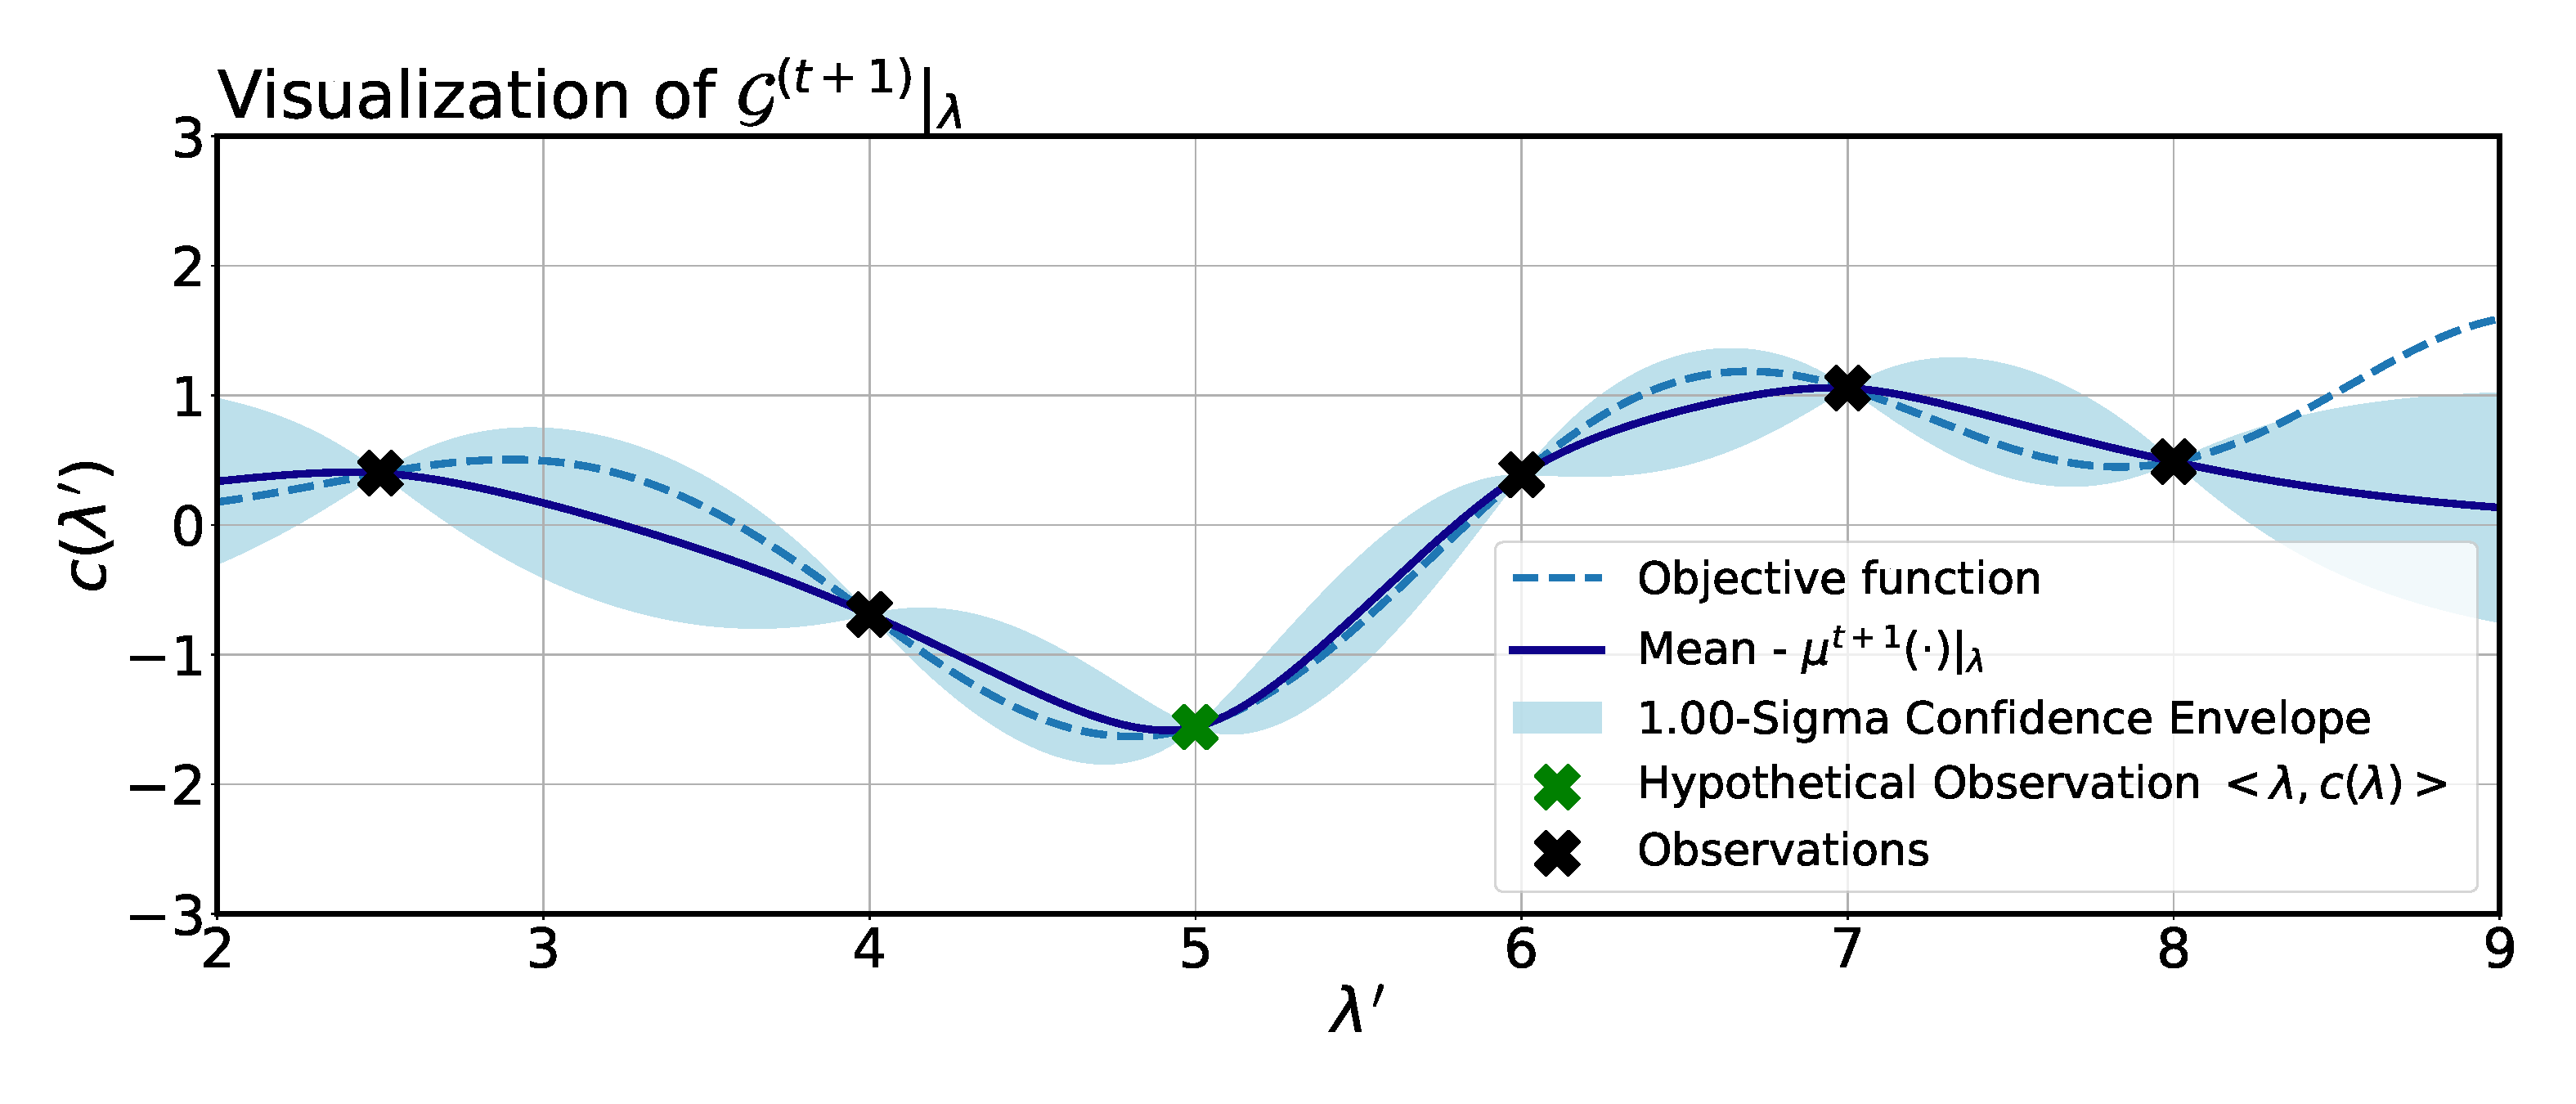
\includegraphics[width=\textwidth, height=0.7\textheight, keepaspectratio=true]{images/acq_func_images/kg/look_ahead_3.pdf}};
    \node<.> [below=0.01\belowcaptionskip of img3, align=center]{If we perform a one-step look-ahead, we would get $\iter[\bocount+1]{\gp}(\cdot\given {\conf})$ for some configuration $\conf$.};
    
    \node<+> (img4) {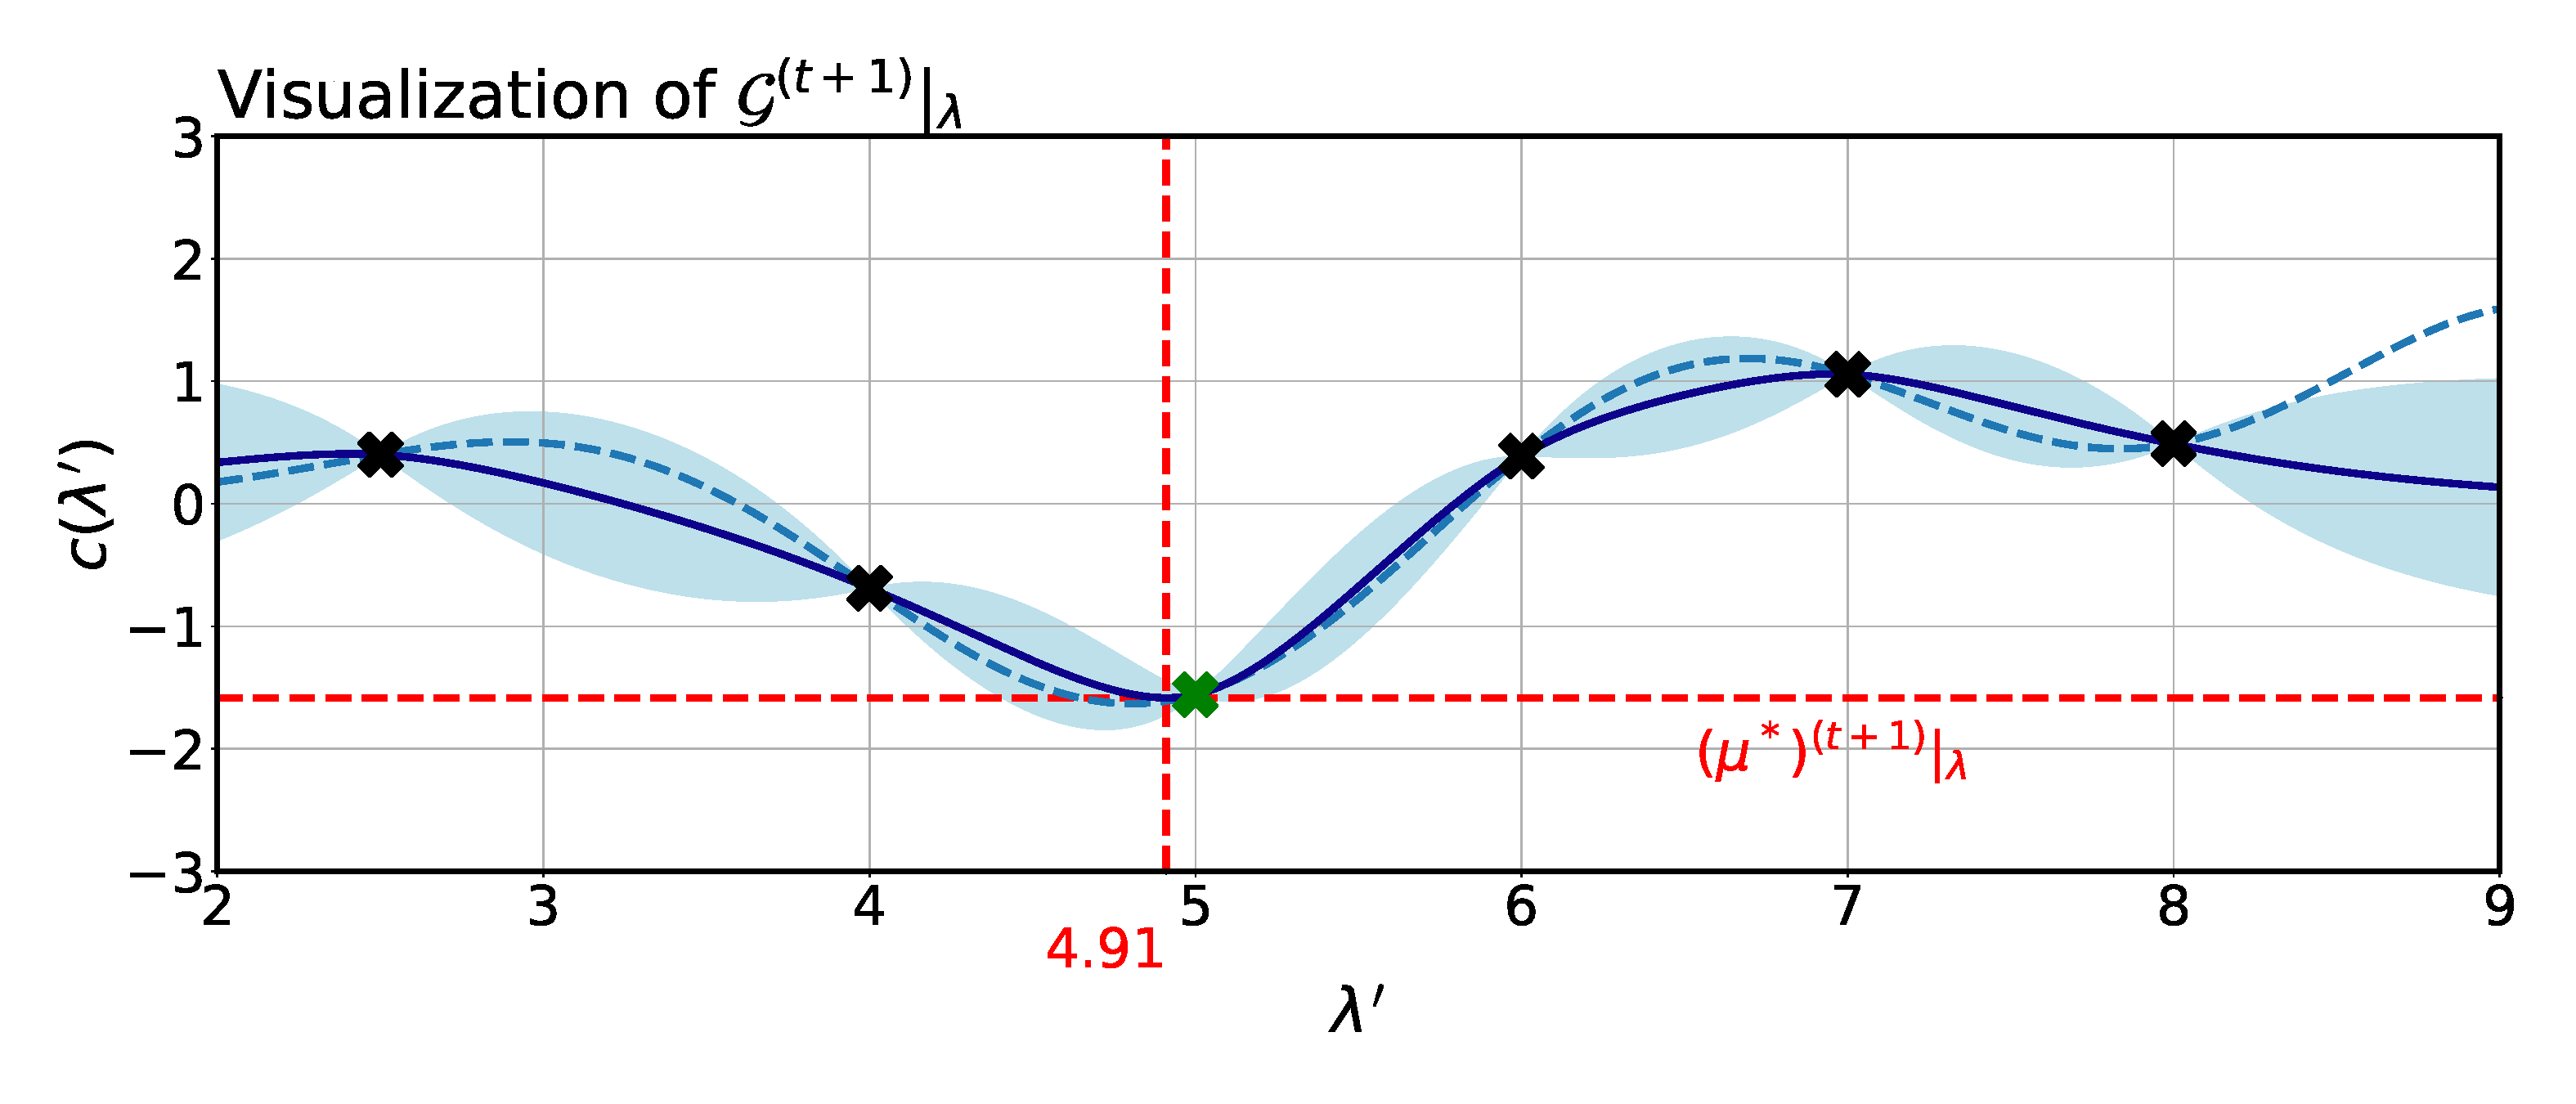
\includegraphics[width=\textwidth, height=0.7\textheight, keepaspectratio=true]{images/acq_func_images/kg/look_ahead_KG_4.pdf}};
    \node<.> [below=-1.0\belowcaptionskip of img4, align=center]{The best risk-neutral choice is again given by the minimum \\of the new conditional mean function - $\iter[\bocount+1]{\left(\mean^*\right)} \given_{\conf}$.};
    
    \node<+> (img5) {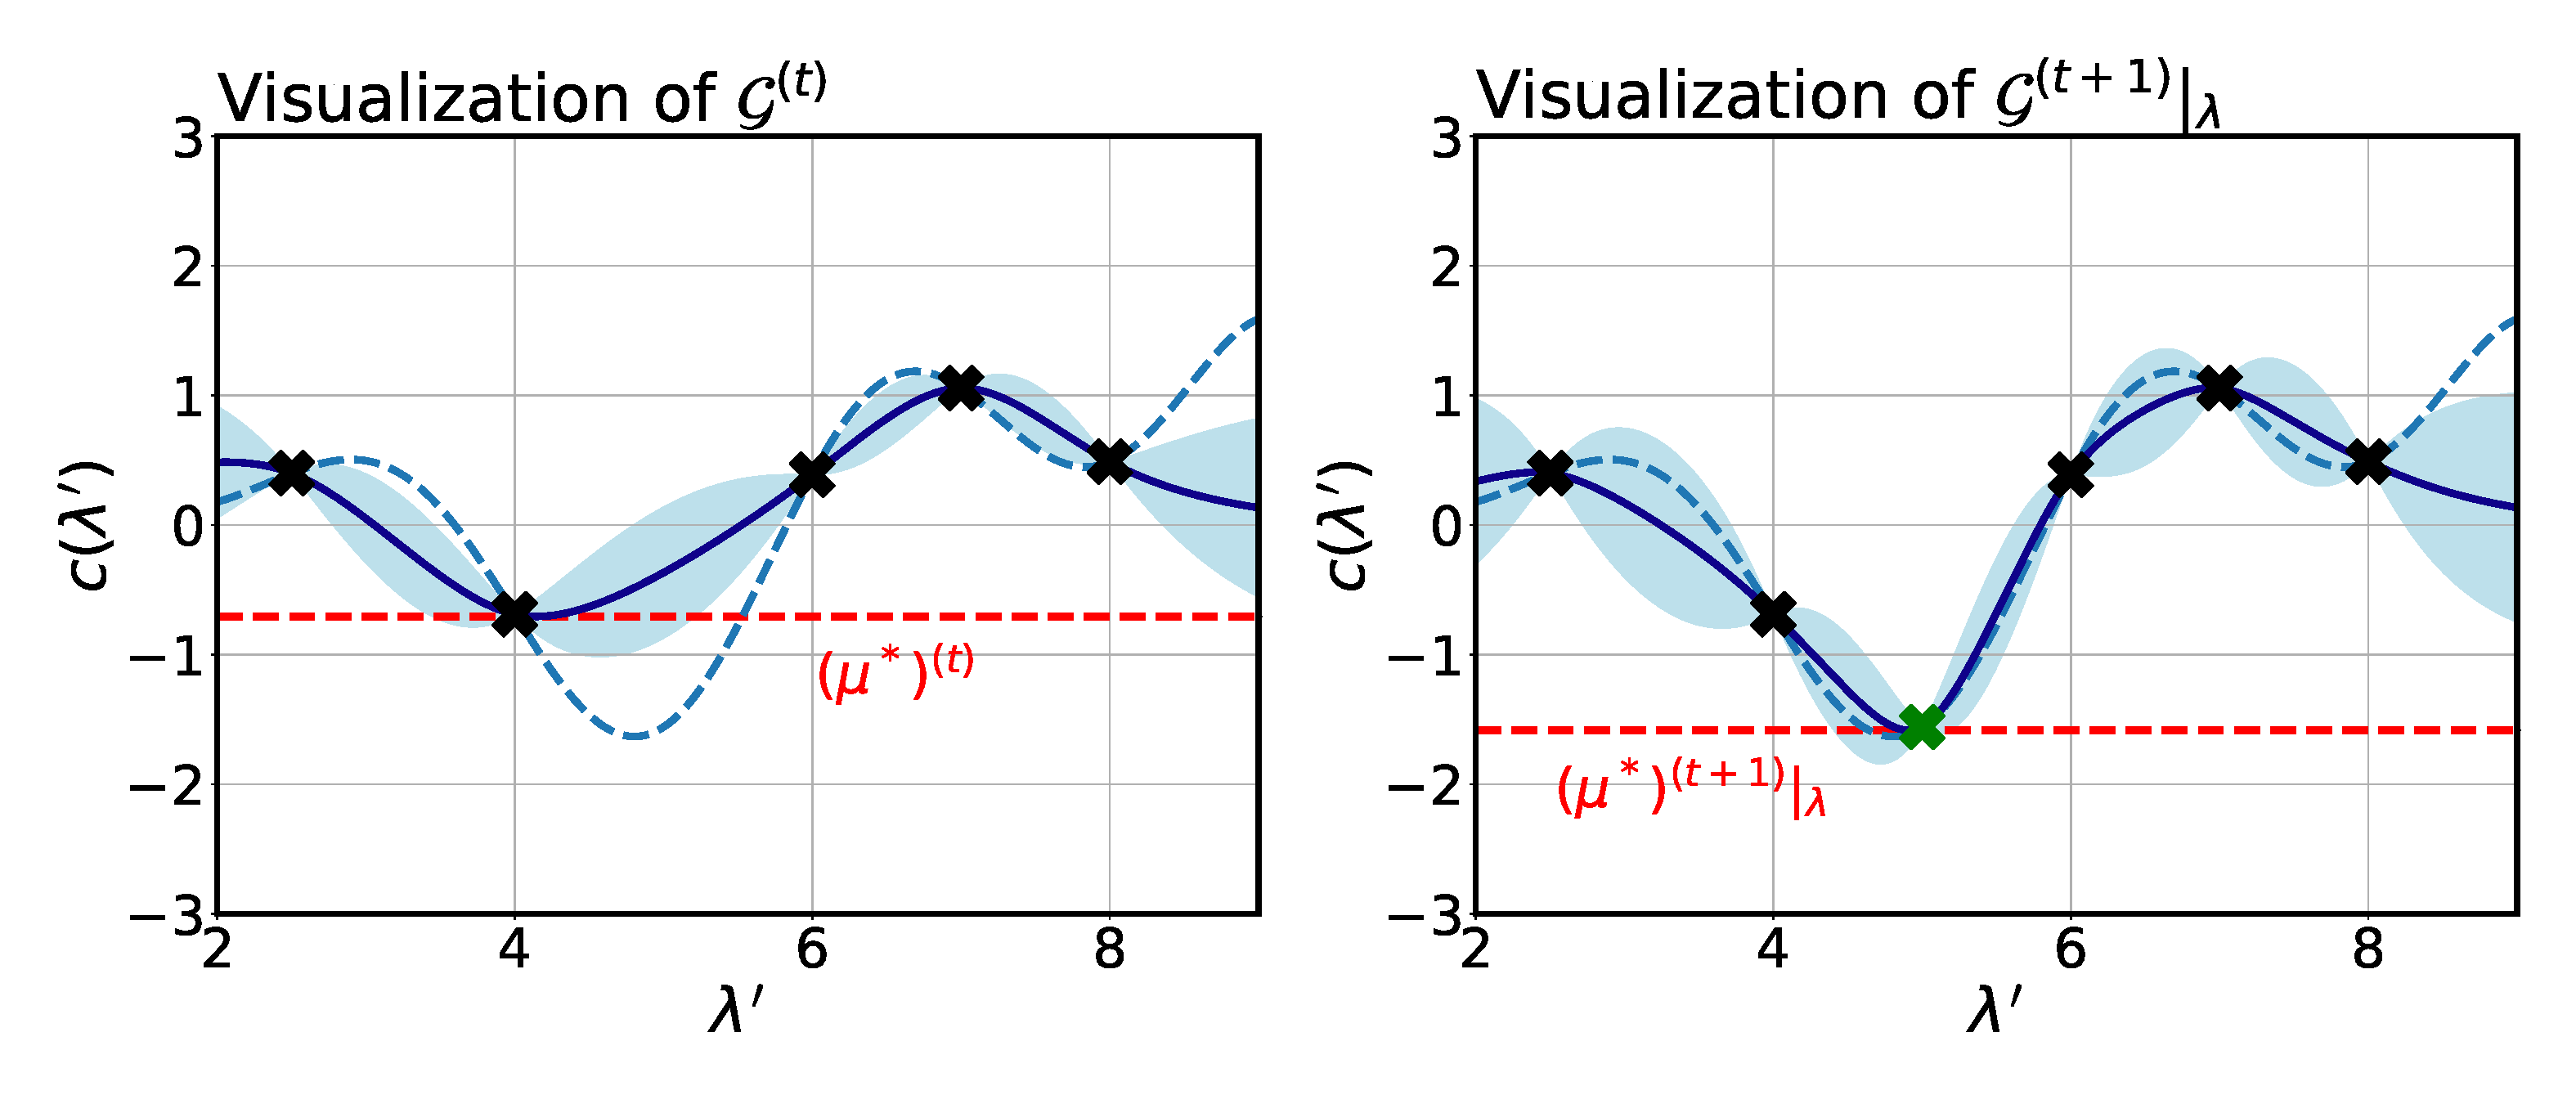
\includegraphics[width=\textwidth, height=0.7\textheight, keepaspectratio=true]{images/acq_func_images/kg/look_ahead_KG_5.pdf}};
    \node<.> [below=-1.0\belowcaptionskip of img5, align=center]{The actual improvement in cost - from $\iter{\left(\mean^*\right)}$ to $\iter[\bocount+1]{\left(\mean^*\right)}$ - cannot be computed \\without evaluation. We compute its expected value i.e. the \emph{Knowledge Gradient}.};
  \end{tikzpicture}
\end{figure}

\end{frame}
%-----------------------------------------------------------------------
\begin{frame}[c]{Computationally Expensive Acquisition Functions - KG}
\framesubtitle{Knowledge Gradient - Choosing a candidate}
\begin{itemize}\belowdisplayskip=1.5em
    \item<+-> Given a GP $\iter{\gp}$ fit on $\iter[\bocount-1]{\dataset}$ on the $\bocount\,$th iteration, we have
    \[
        \iter{\left(\mean^*\right)} = \min_{\conf'\in\pcs}\,\iter{\mean}\left(\conf'\big|\iter[\bocount-1]{\dataset}\right)
    \]
    
    \item<+-> If we choose a candidate $\bonextsample=\conf$ to evaluate $\cost(\cdot)$ at,
    \[
        \left.\iter{\dataset}\right|_{\conf} = \iter[\bocount-1]{\dataset}\cup\left\{\left\langle\bonextsample,\,\bonextobs\right\rangle\big|\bonextsample=\conf\right\}
    \]
    
    \item <+-> Thus, if we hypothesize about the $\bocount+1\,$th iteration, we would get
    \[
        \begin{split}
        \left.\iter[\bocount+1]{\left(\mean^*\right)} \right|_{\conf} 
        &= \min_{\conf'\in\pcs} \iter[\bocount+1]{\mean} \left(\conf'\big| \iter{\dataset},\bonextsample=\conf \right)\\
        %&= \min_{\conf'\in\pcs} \iter[\bocount+1]{\mean} \left(\conf'\big| \iter[\bocount-1]{\dataset},\conf,\obs \right)\\
        \end{split}
    \]
\end{itemize}
\comment{Source:https://arxiv.org/pdf/1807.02811.pdf}
\end{frame}
%-----------------------------------------------------------------------
\begin{frame}[c]{Computationally Expensive Acquisition Functions - KG}
\framesubtitle{Knowledge Gradient - Choosing a candidate}
\begin{itemize}\belowdisplayskip=1.5em
    \item<+->In a risk-neutral setting, $\iter{\left(\mean^*\right)}$ and $\left.\iter[\bocount+1]{\left(\mean^*\right)}\right|_{\conf}$ are the global optima for $\iter{\mean}$ and $\left.\iter[\bocount+1]{\mean}\right|_{\conf}$ respectively.
    
    \item<+-> Thus, the conditional improvement in the cost is 
    \[
        \left.\iter{I}\right|_{\conf}=\iter{\left(\mean^*\right)} - \left.\iter[\bocount+1]{\left(\mean^*\right)} \right|_{\bonextsample=\conf}
    \]
    
    \item<+-> We cannot directly compute this improvement without performing an evaluation, but we can compute its expected value, which we call \emph{Knowledge Gradient}.
    \lit{\href{https://arxiv.org/pdf/1807.02811.pdf}{Frazier 2018}}
\end{itemize}
\end{frame}
%-----------------------------------------------------------------------
\begin{frame}[c]{Computationally Expensive Acquisition Functions - KG}
\framesubtitle{Knowledge Gradient - Choosing a candidate}
\begin{itemize}\belowdisplayskip=1.5em
    
    \item<+-> Thus,
    \[
    \begin{split}
        \iter{\acq}_{KG}(\conf) 
        &= \E\left[ \iter{\left(\mean^*\right)} - \left. \iter[\bocount+1]{\left(\mean^*\right)} \right|_{\bonextsample=\conf} \right]\\
        &=\min_{\conf'\in\pcs} \, \iter{\mean} \left(\conf' \big| \iter[\bocount-1]{\dataset} \right)
        - \E_{\tilde{\cost} \sim \iter[\bocount]{\surro(\lambda)}}
        %{p\left(\obs\big|\iter[\bocount-1]{\dataset},\conf\right)}
        \left[\min_{\conf'\in\pcs}\iter[\bocount+1]{\mean}\left(\conf'\given{\iter[\bocount-1]{\dataset} \cup \left\{\left\langle\conf, \tilde{\cost} \right\rangle \right\}}\right)\right]
    \end{split}
    \]
    
    \item<+-> Finally, 
    \[
    \text{Choose}\,\boxed{\bonextsample = \argmax_{\conf\in\pcs}(\iter{\acq}_{KG}(\conf))}
    \]
    \comment{\lit{\href{https://arxiv.org/pdf/1807.02811.pdf}{Frazier 2018}}}
\end{itemize}
\end{frame}
%-----------------------------------------------------------------------
\begin{frame}[c]{Computationally Expensive Acquisition Functions - ES}
\framesubtitle{Entropy Search - Choosing a candidate}
\begin{itemize}
    \item<+-> Idea: Evaluate $\conf$ which reduces our uncertainty about the location of $\optconf$.
    \item<+-> Do this by minimizing the entropy of the distribution of the lowation of the minimum: $\mathcal{H}(p_{min})$
    \item<+-> $p_{min}(\conf^*|\dataset) = p(\conf^* \in \argmin_{\conf' \in \pcs} (\surro(\conf') | \dataset))$
    \item<+-> We define the acquisition function as 
    \[
    \begin{split}
      \iter{\acq}_{ES}(\conf,\dataset) = \mathcal{H}\left(p_{min}(\conf^*)|\dataset \right) - \E_{\tilde{\cost} \sim \iter[\bocount]{\surro(\conf)}}\left[\mathcal{H} \left( p_{min}(\conf^*)|\dataset \cup \left\{ \left\langle \conf, \tilde{\cost} \right\rangle \right\} \right)\right]
    \end{split}
    \]
    \item<+-> Entropy search contains a similar look-ahead as knoledge gradient
    \item<+-> And as always, 
    \[
    \text{Choose}\,\boxed{\bonextsample = \argmax_{\conf\in\pcs}(\iter{\acq}_{ES}(\conf))}
    \]
\end{itemize}
\comment{Source:\lit{\href{Frazier 2018}{https://arxiv.org/pdf/1807.02811.pdf}}}
\end{frame}
%-----------------------------------------------------------------------
\begin{frame}[c]{Computationally Expensive Acquisition Functions - ES}
\framesubtitle{Entropy Search - Concept}

\begin{figure}
  \centering
  \begin{tikzpicture}
    \node<+> (img1) {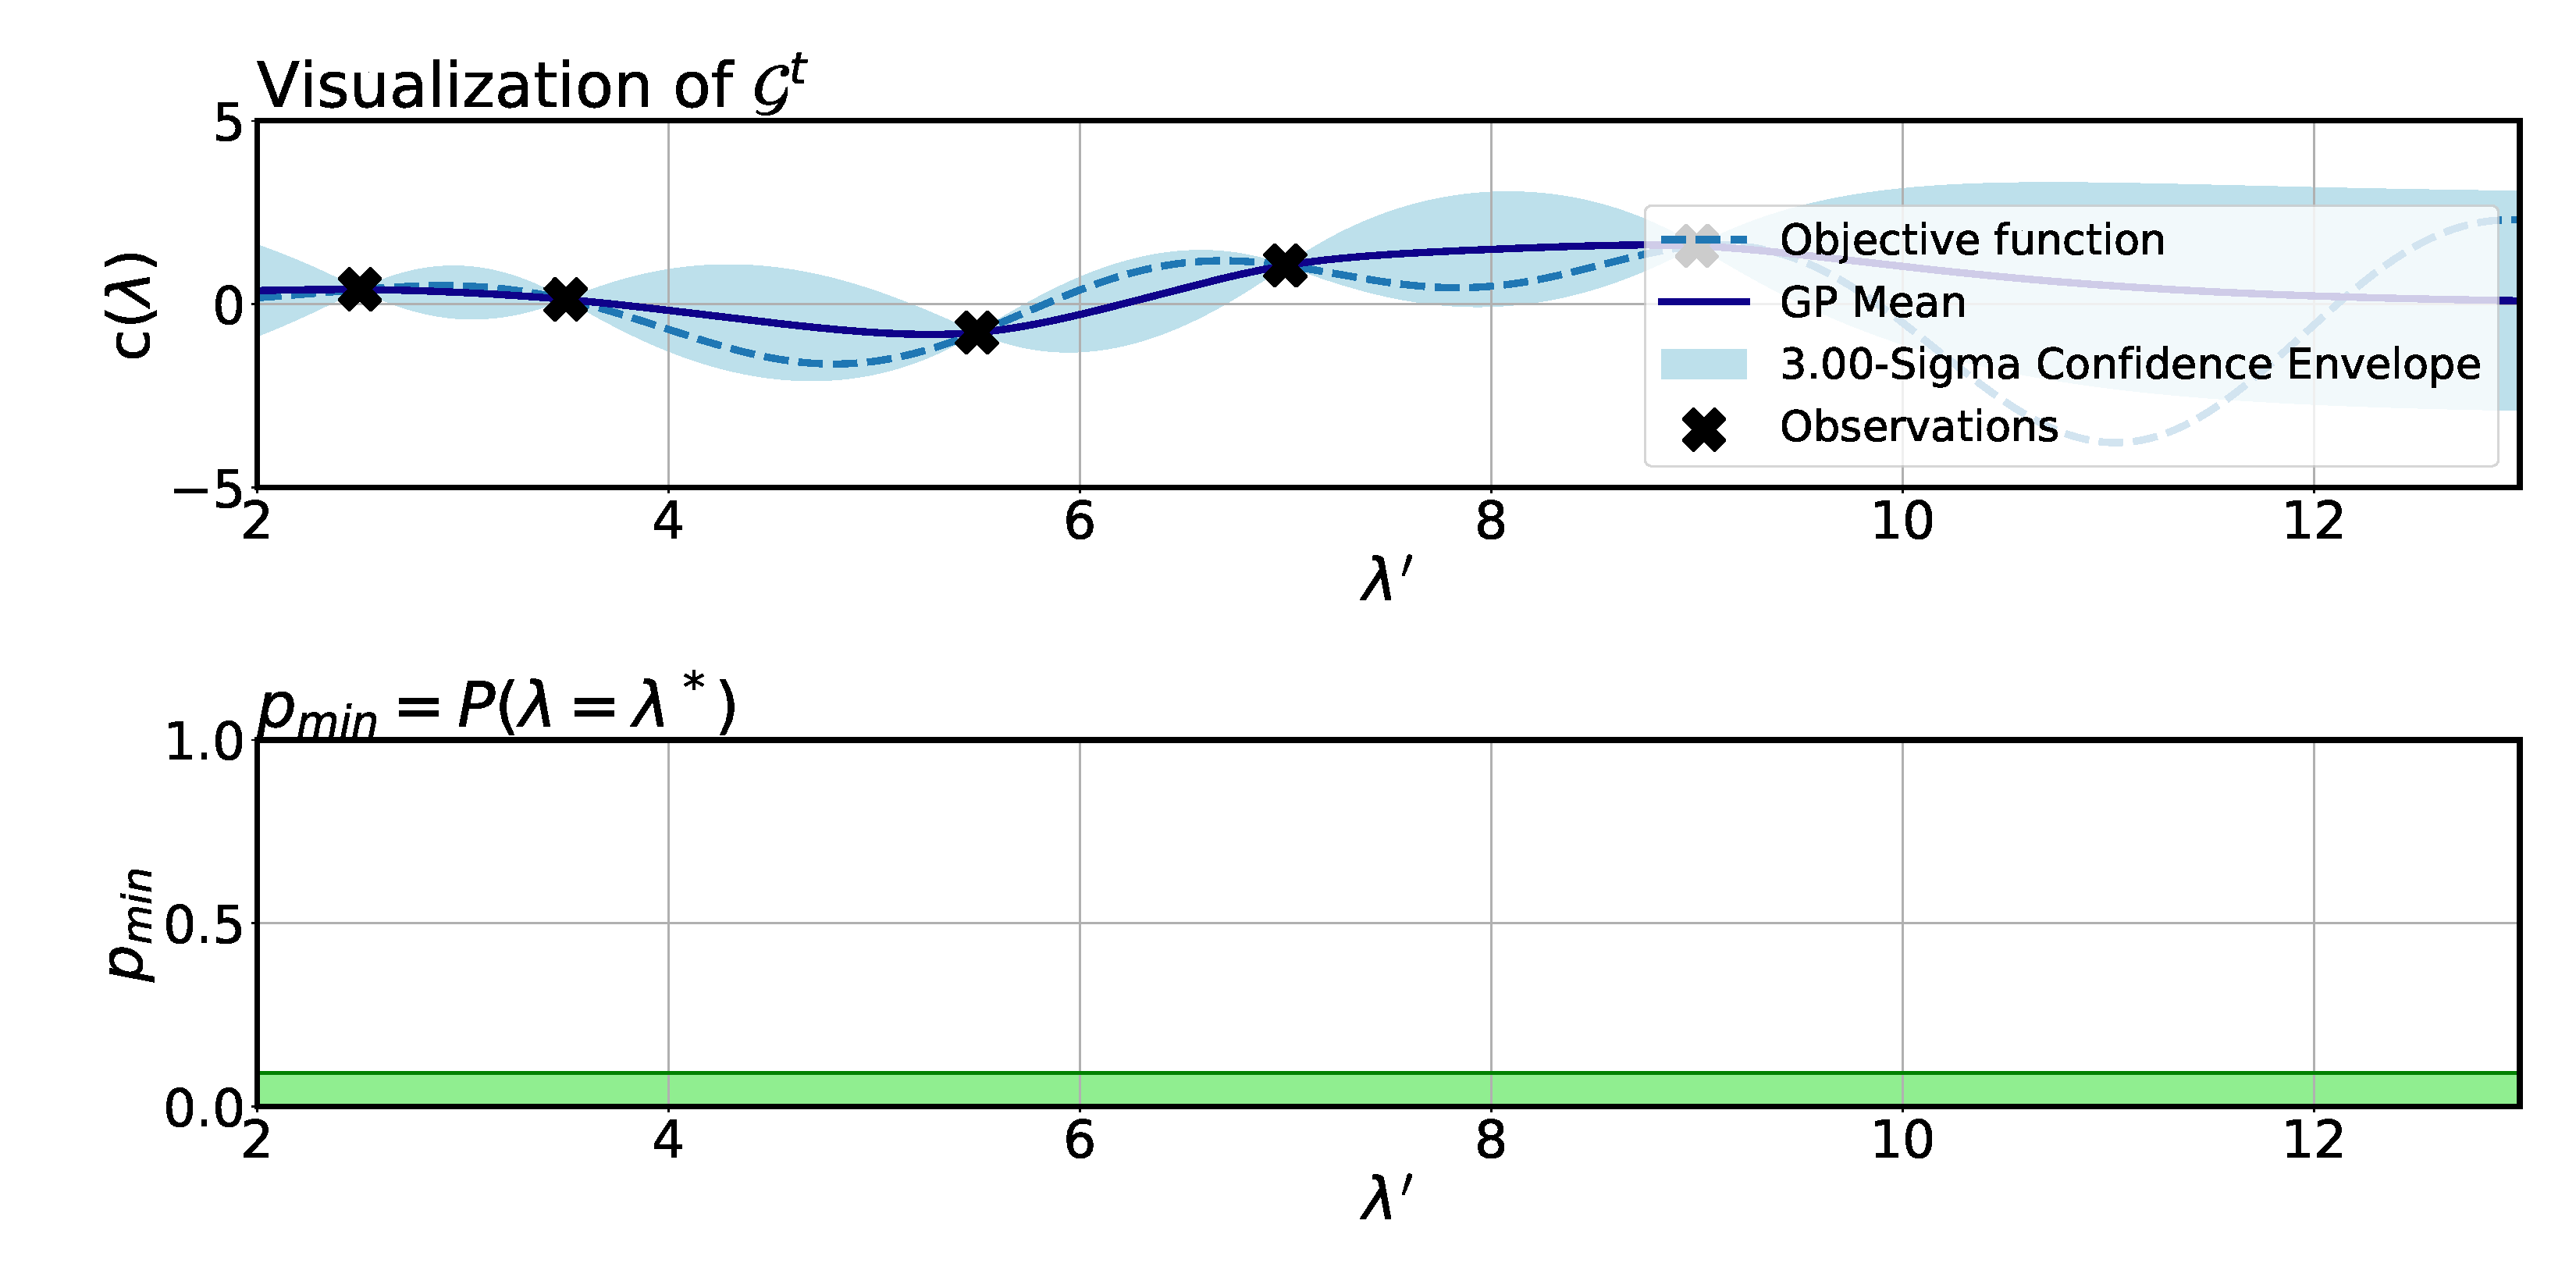
\includegraphics[width=\linewidth, height=0.7\textheight, keepaspectratio=true]{images/acq_func_images/es/es_1.pdf}};
    \node<.> [below=-1.0\belowcaptionskip of img1, align=center]{We consider the global optimum's position to be a random variable $\conf^*$, \\ so each configuration $\conf$ can be assigned a probability $p_{min}=P(\conf=\conf^*)$.};
    
    \node<+> (img2) {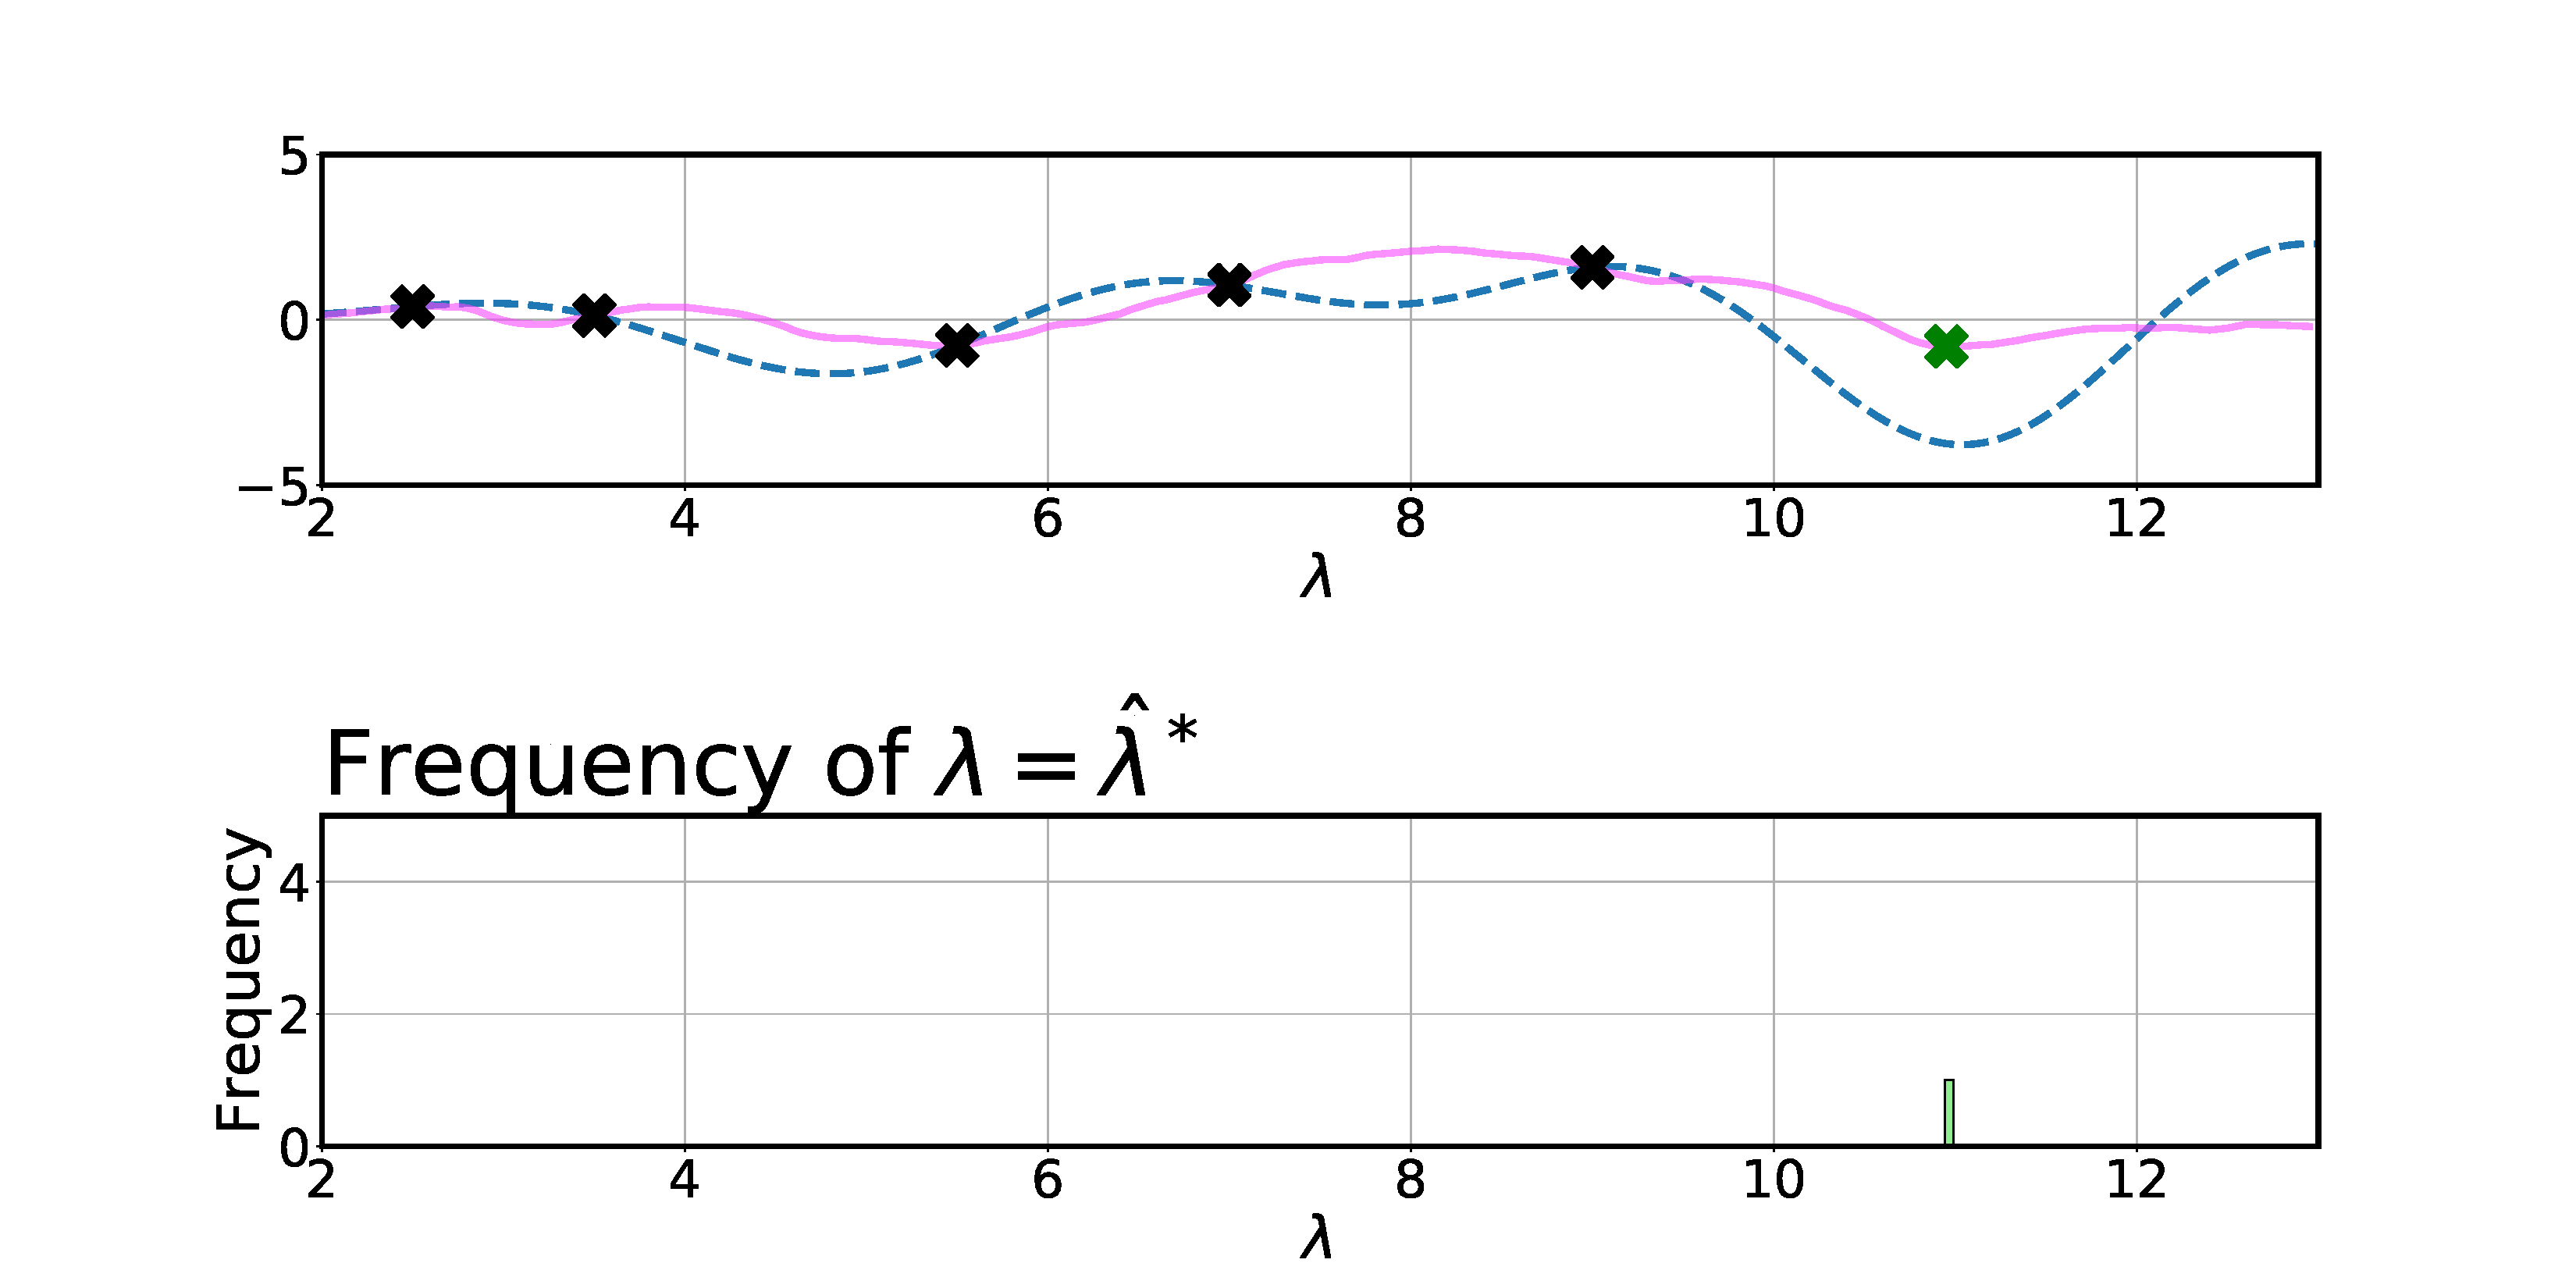
\includegraphics[width=\linewidth, height=0.7\textheight, keepaspectratio=true]{images/acq_func_images/es/es_2.pdf}};
    \node<.> [below=-1.0\belowcaptionskip of img2, align=center]{The minimizing configuration $\hat{\conf}$ of a sample from the GP $\iter{\gp}$ \\provides some evidence for where $\conf^*$ may lie.};
    
    \node<+> (img3) {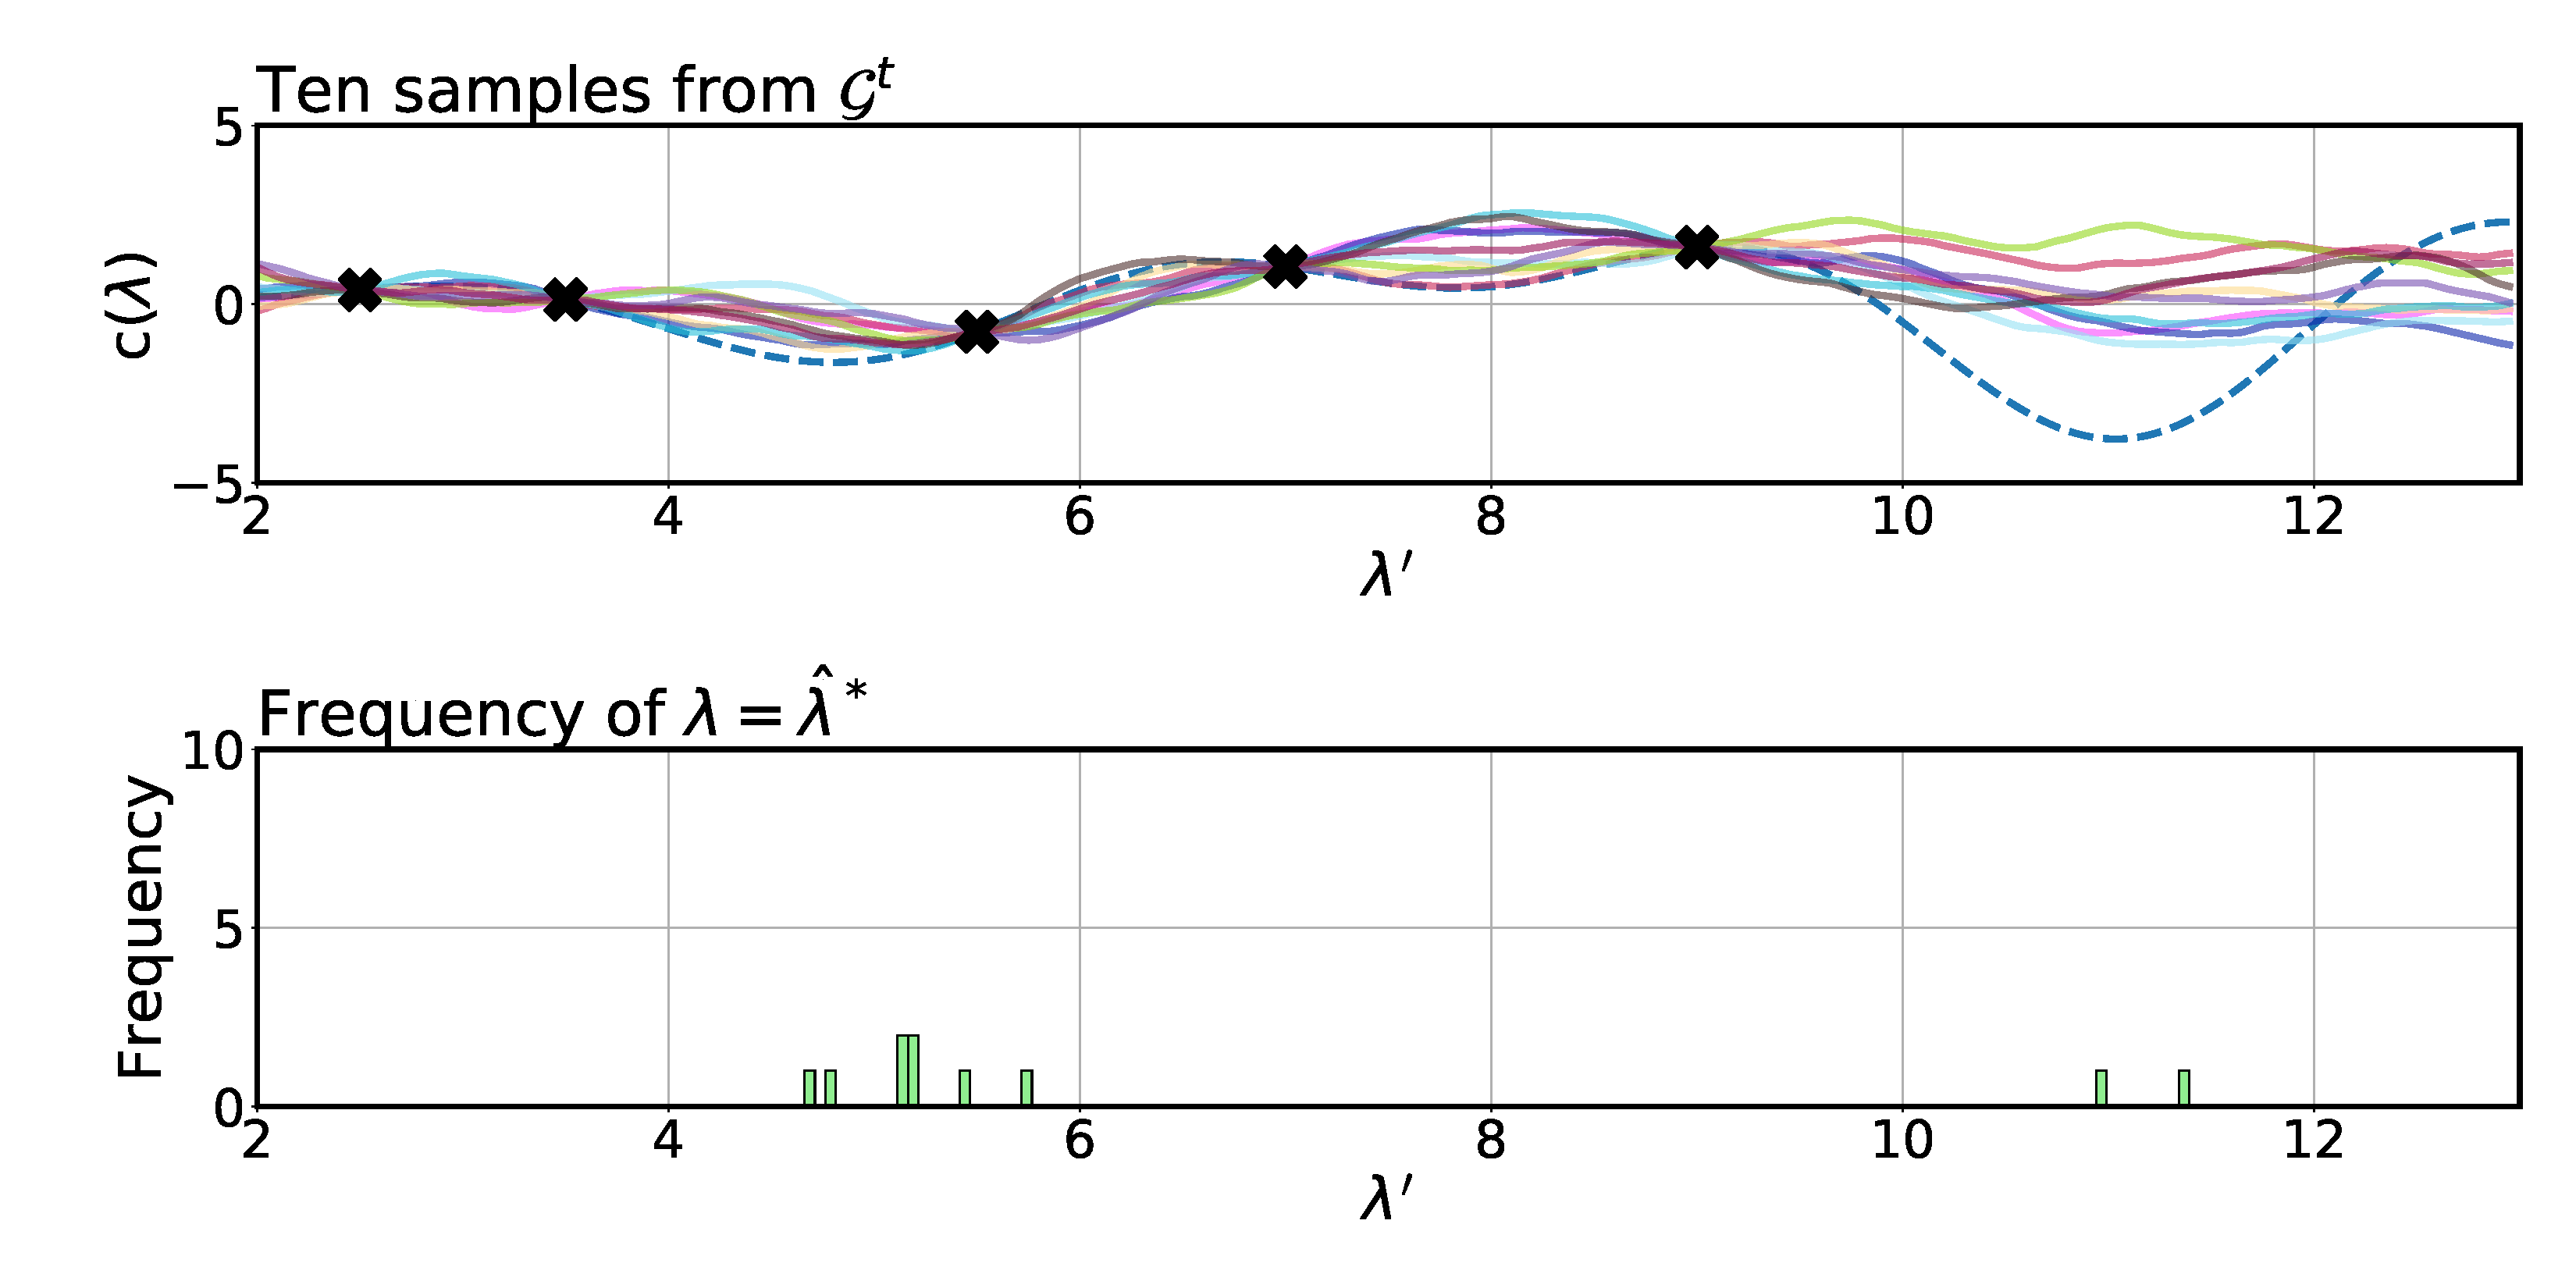
\includegraphics[width=\linewidth, height=0.7\textheight, keepaspectratio=true]{images/acq_func_images/es/es_3.pdf}};
    \node<.> [below=-1.0\belowcaptionskip of img3, align=center]{Each new sample provides more information about where the global minimum lies - \\i.e. has an associated \emph{information gain}.};
    
    \node<+> (img4) {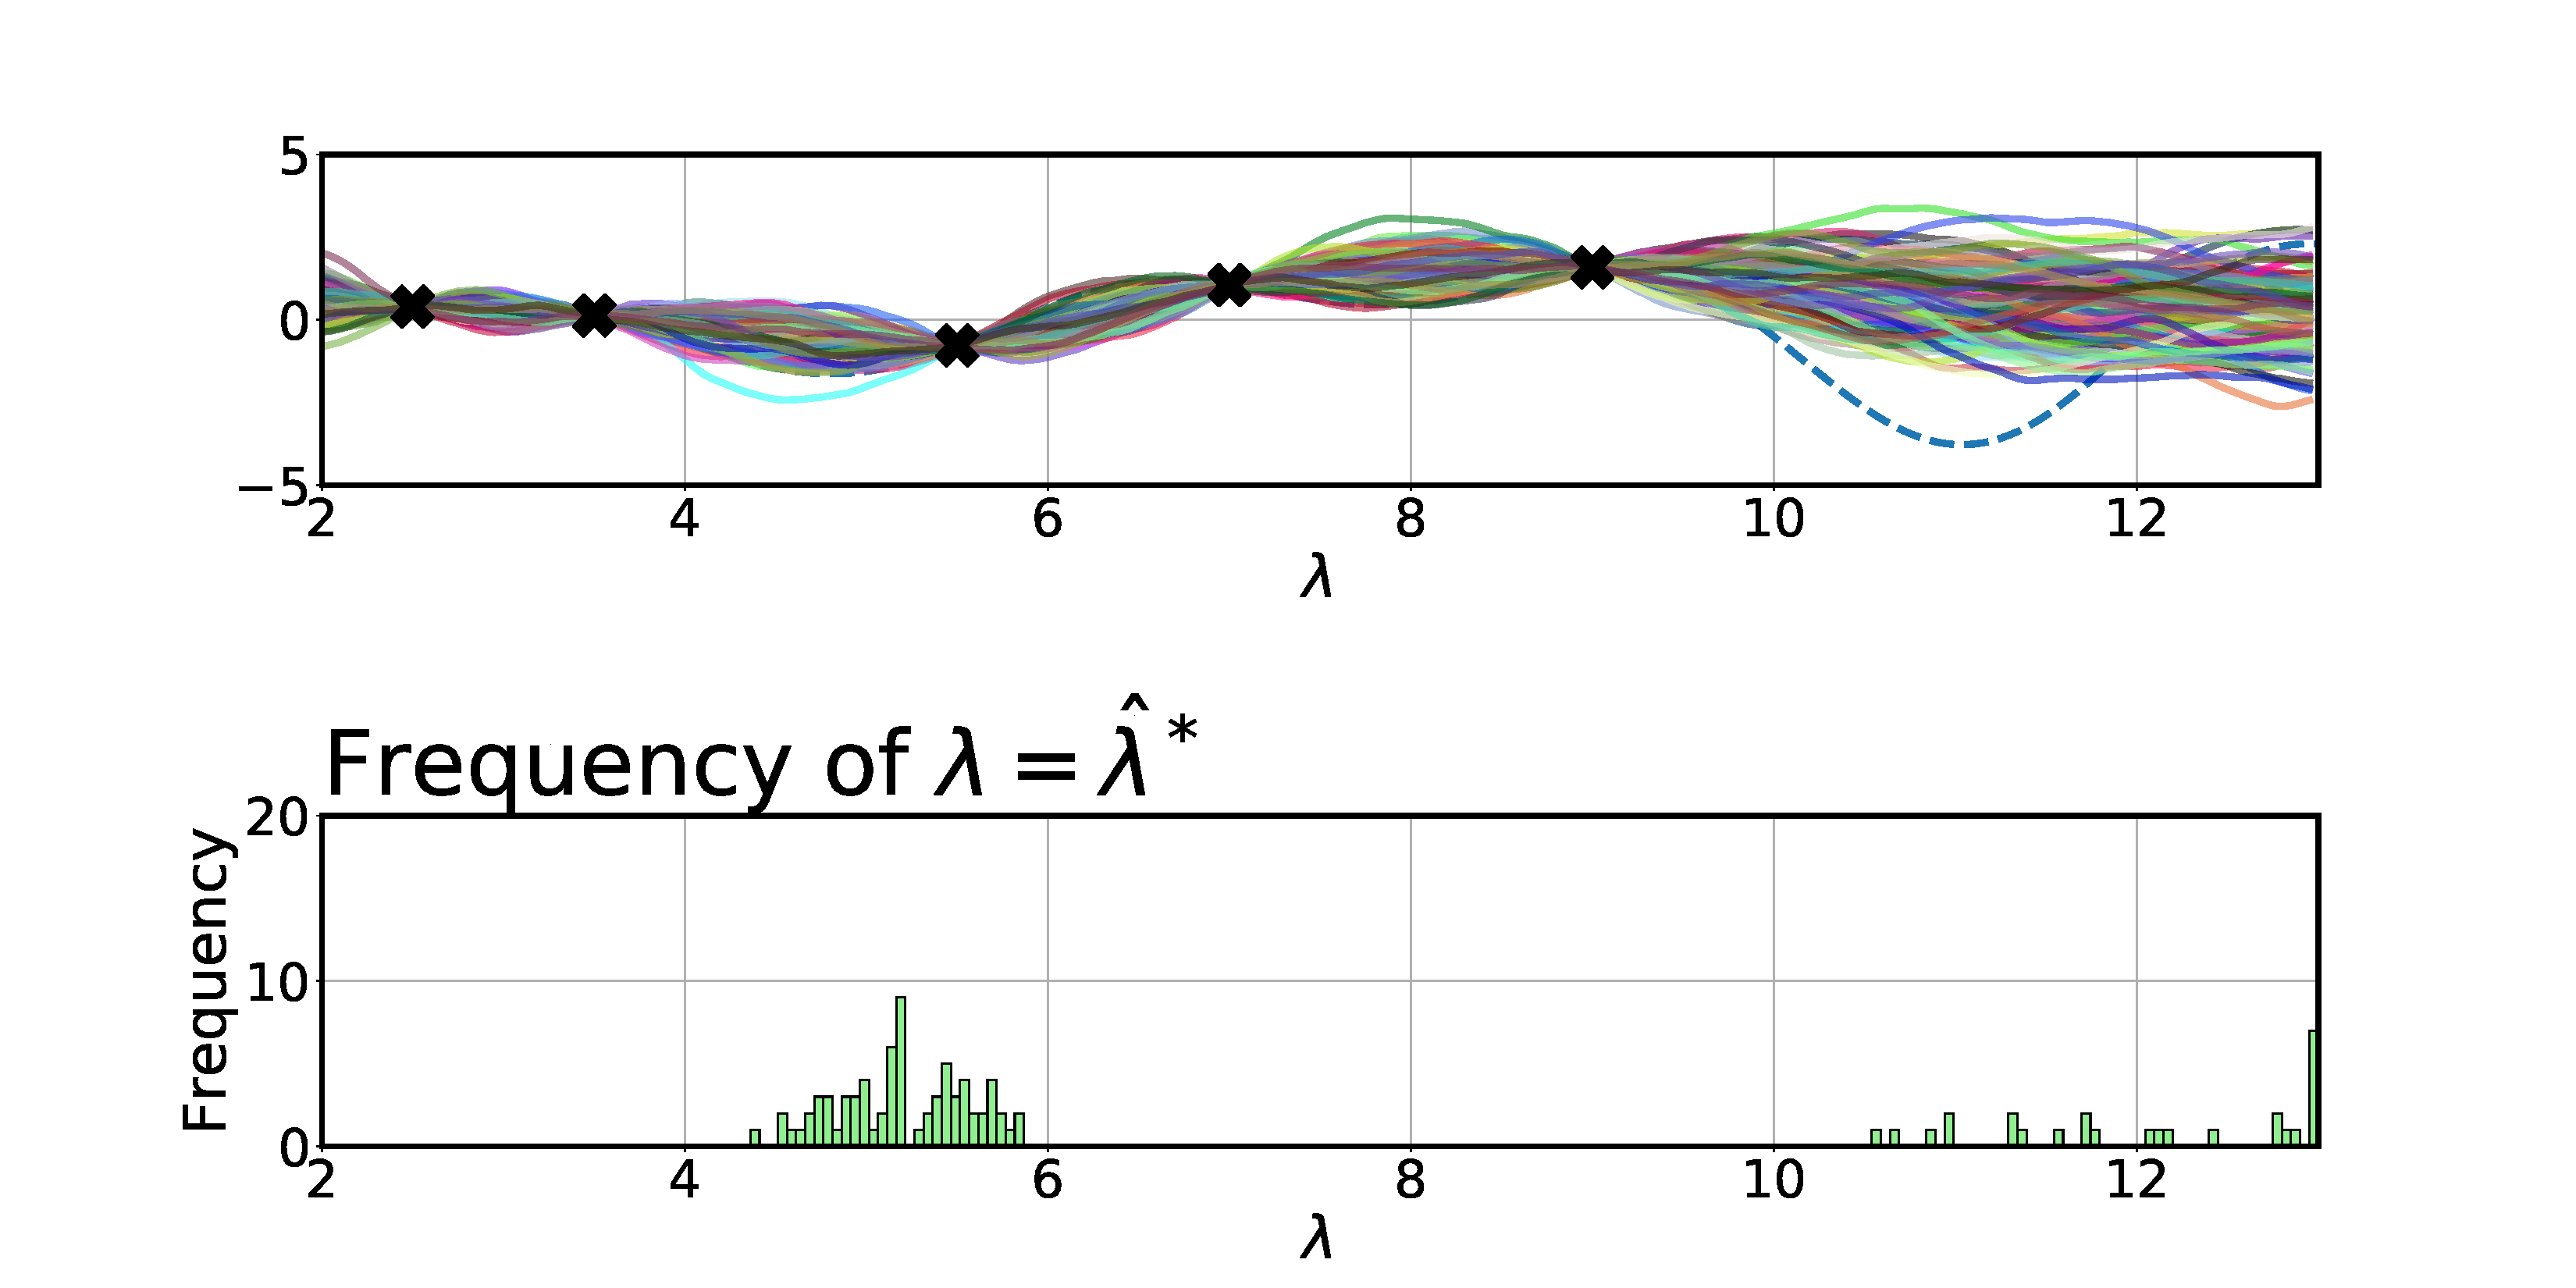
\includegraphics[width=\linewidth, height=0.7\textheight, keepaspectratio=true]{images/acq_func_images/es/es_4.pdf}};
    \node<.> [below=-1.0\belowcaptionskip of img4, align=center]{After many such samples, \\we can narrow down the approximate location of the global minimum.};
    
    \node<+> (img5) {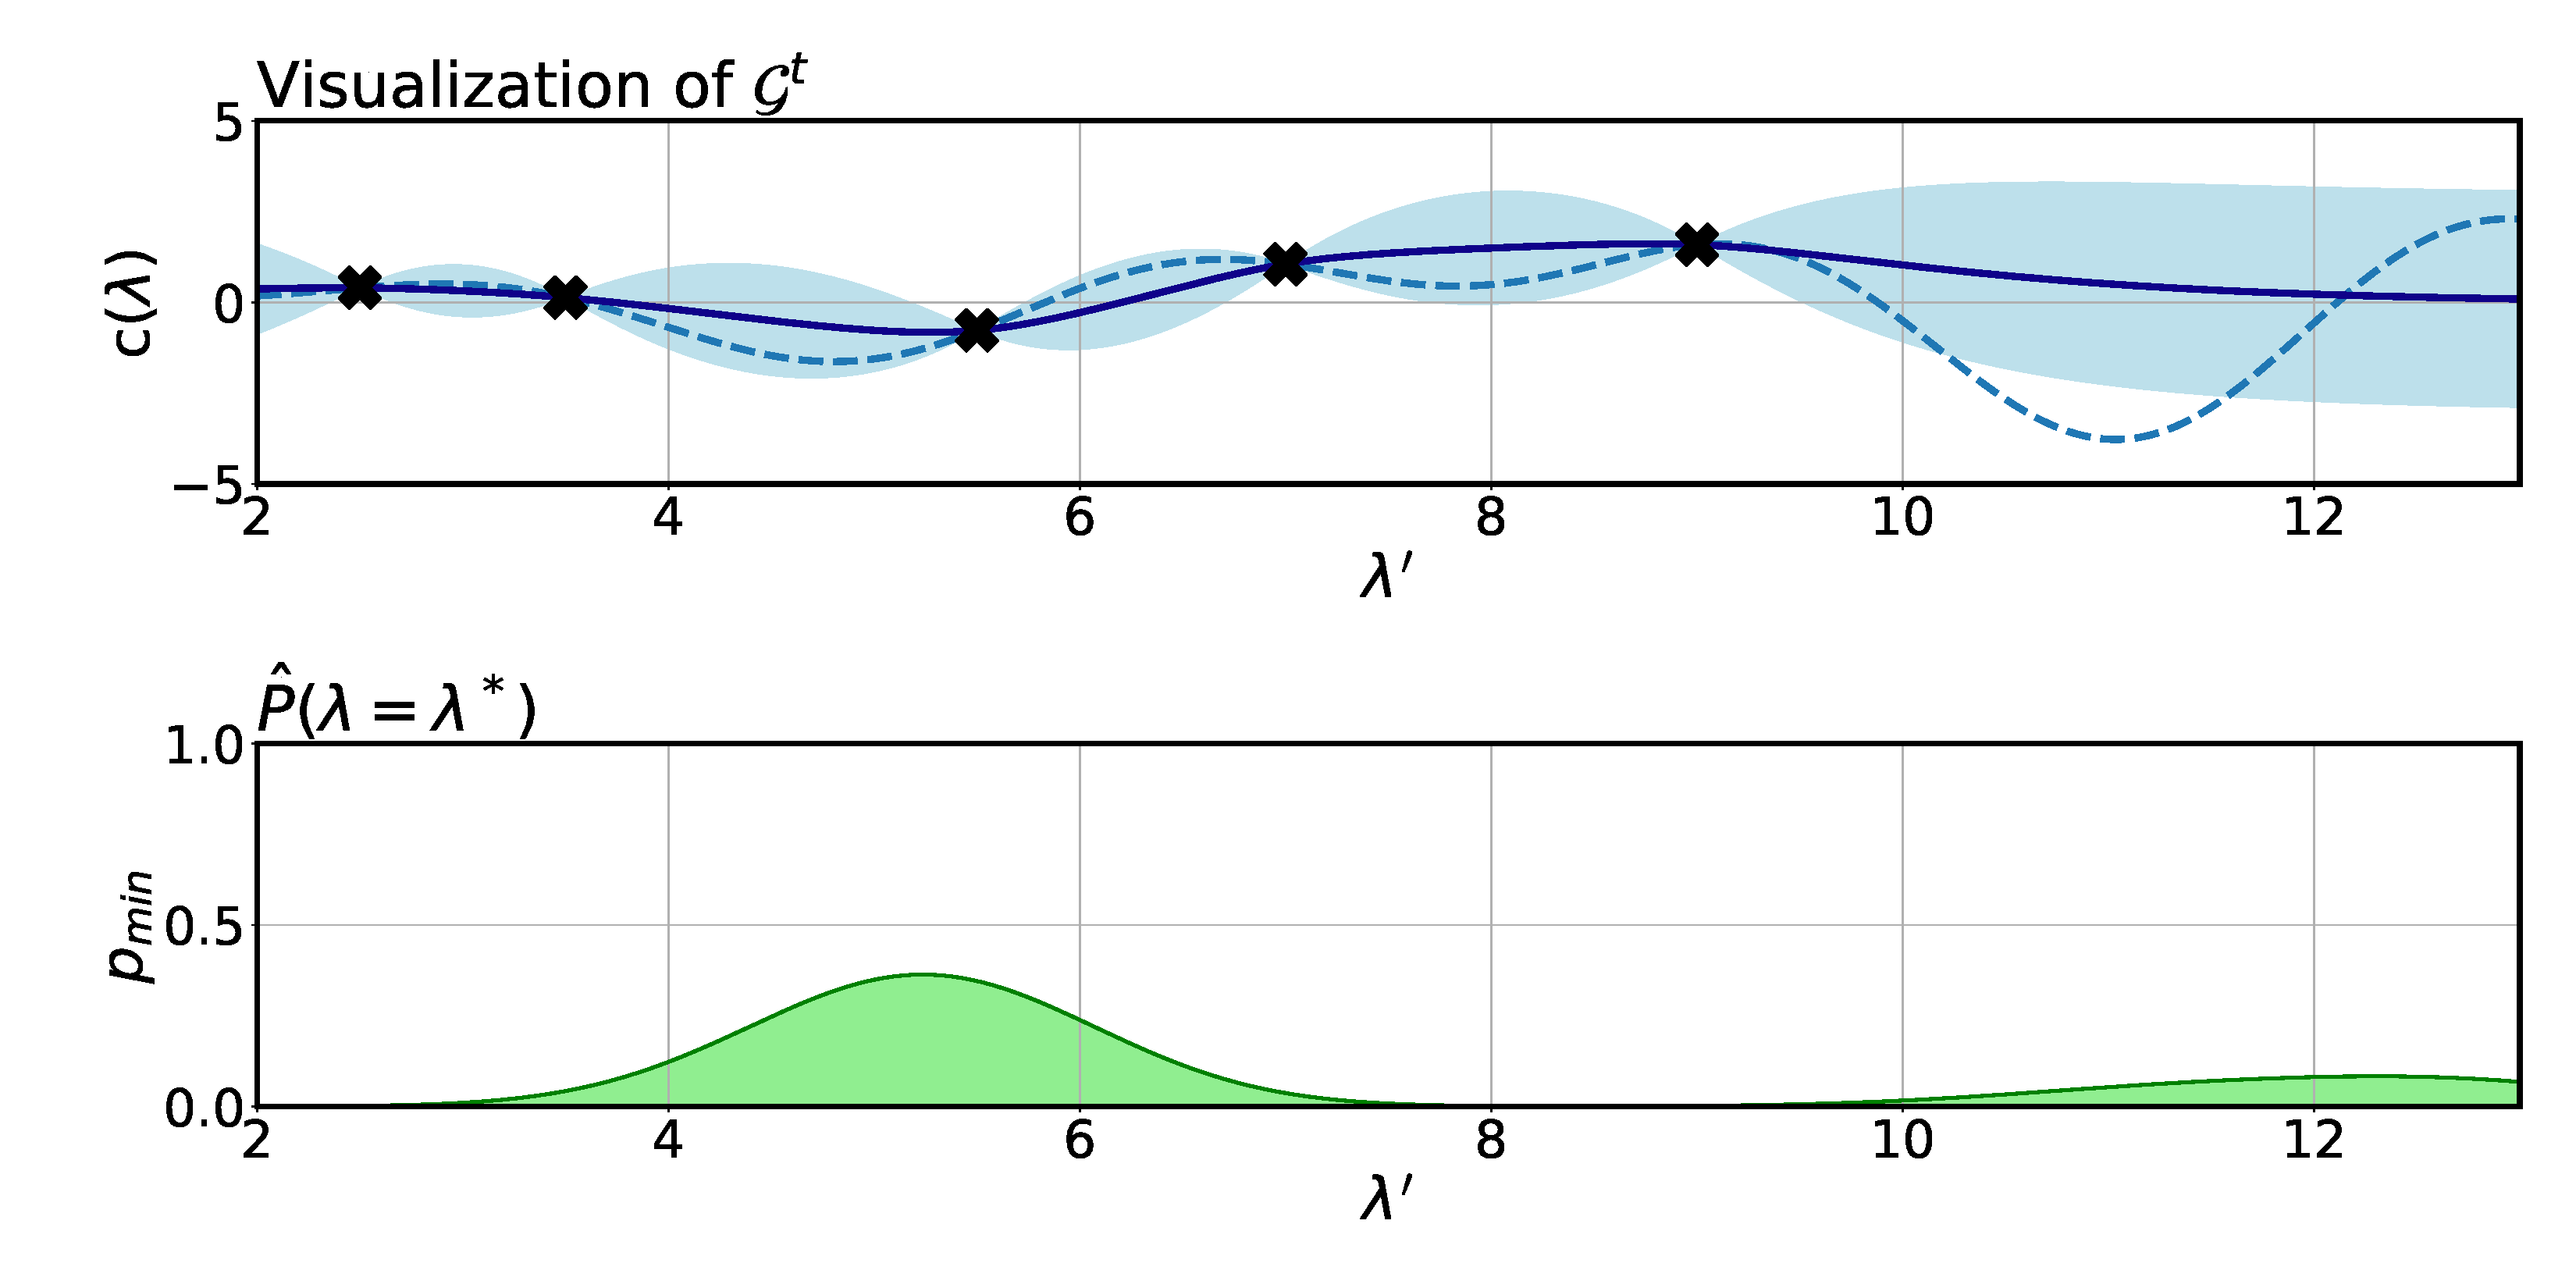
\includegraphics[width=\linewidth, height=0.7\textheight, keepaspectratio=true]{images/acq_func_images/es/es_5.pdf}};
    \node<.> [below=-1.0\belowcaptionskip of img5, align=center]{An approximate probability distribution for $p_{min}$ can now be generated.};
    \comment{Since the aim was to illustrate a concept, the underlying code for these plots used simplified max-value entropy search, and the final PDF was generated using Kernel Density Estimation, thus leading to an artifact at the right edge where a very high bin value was "lost".}
    
    \node<+> (img6) {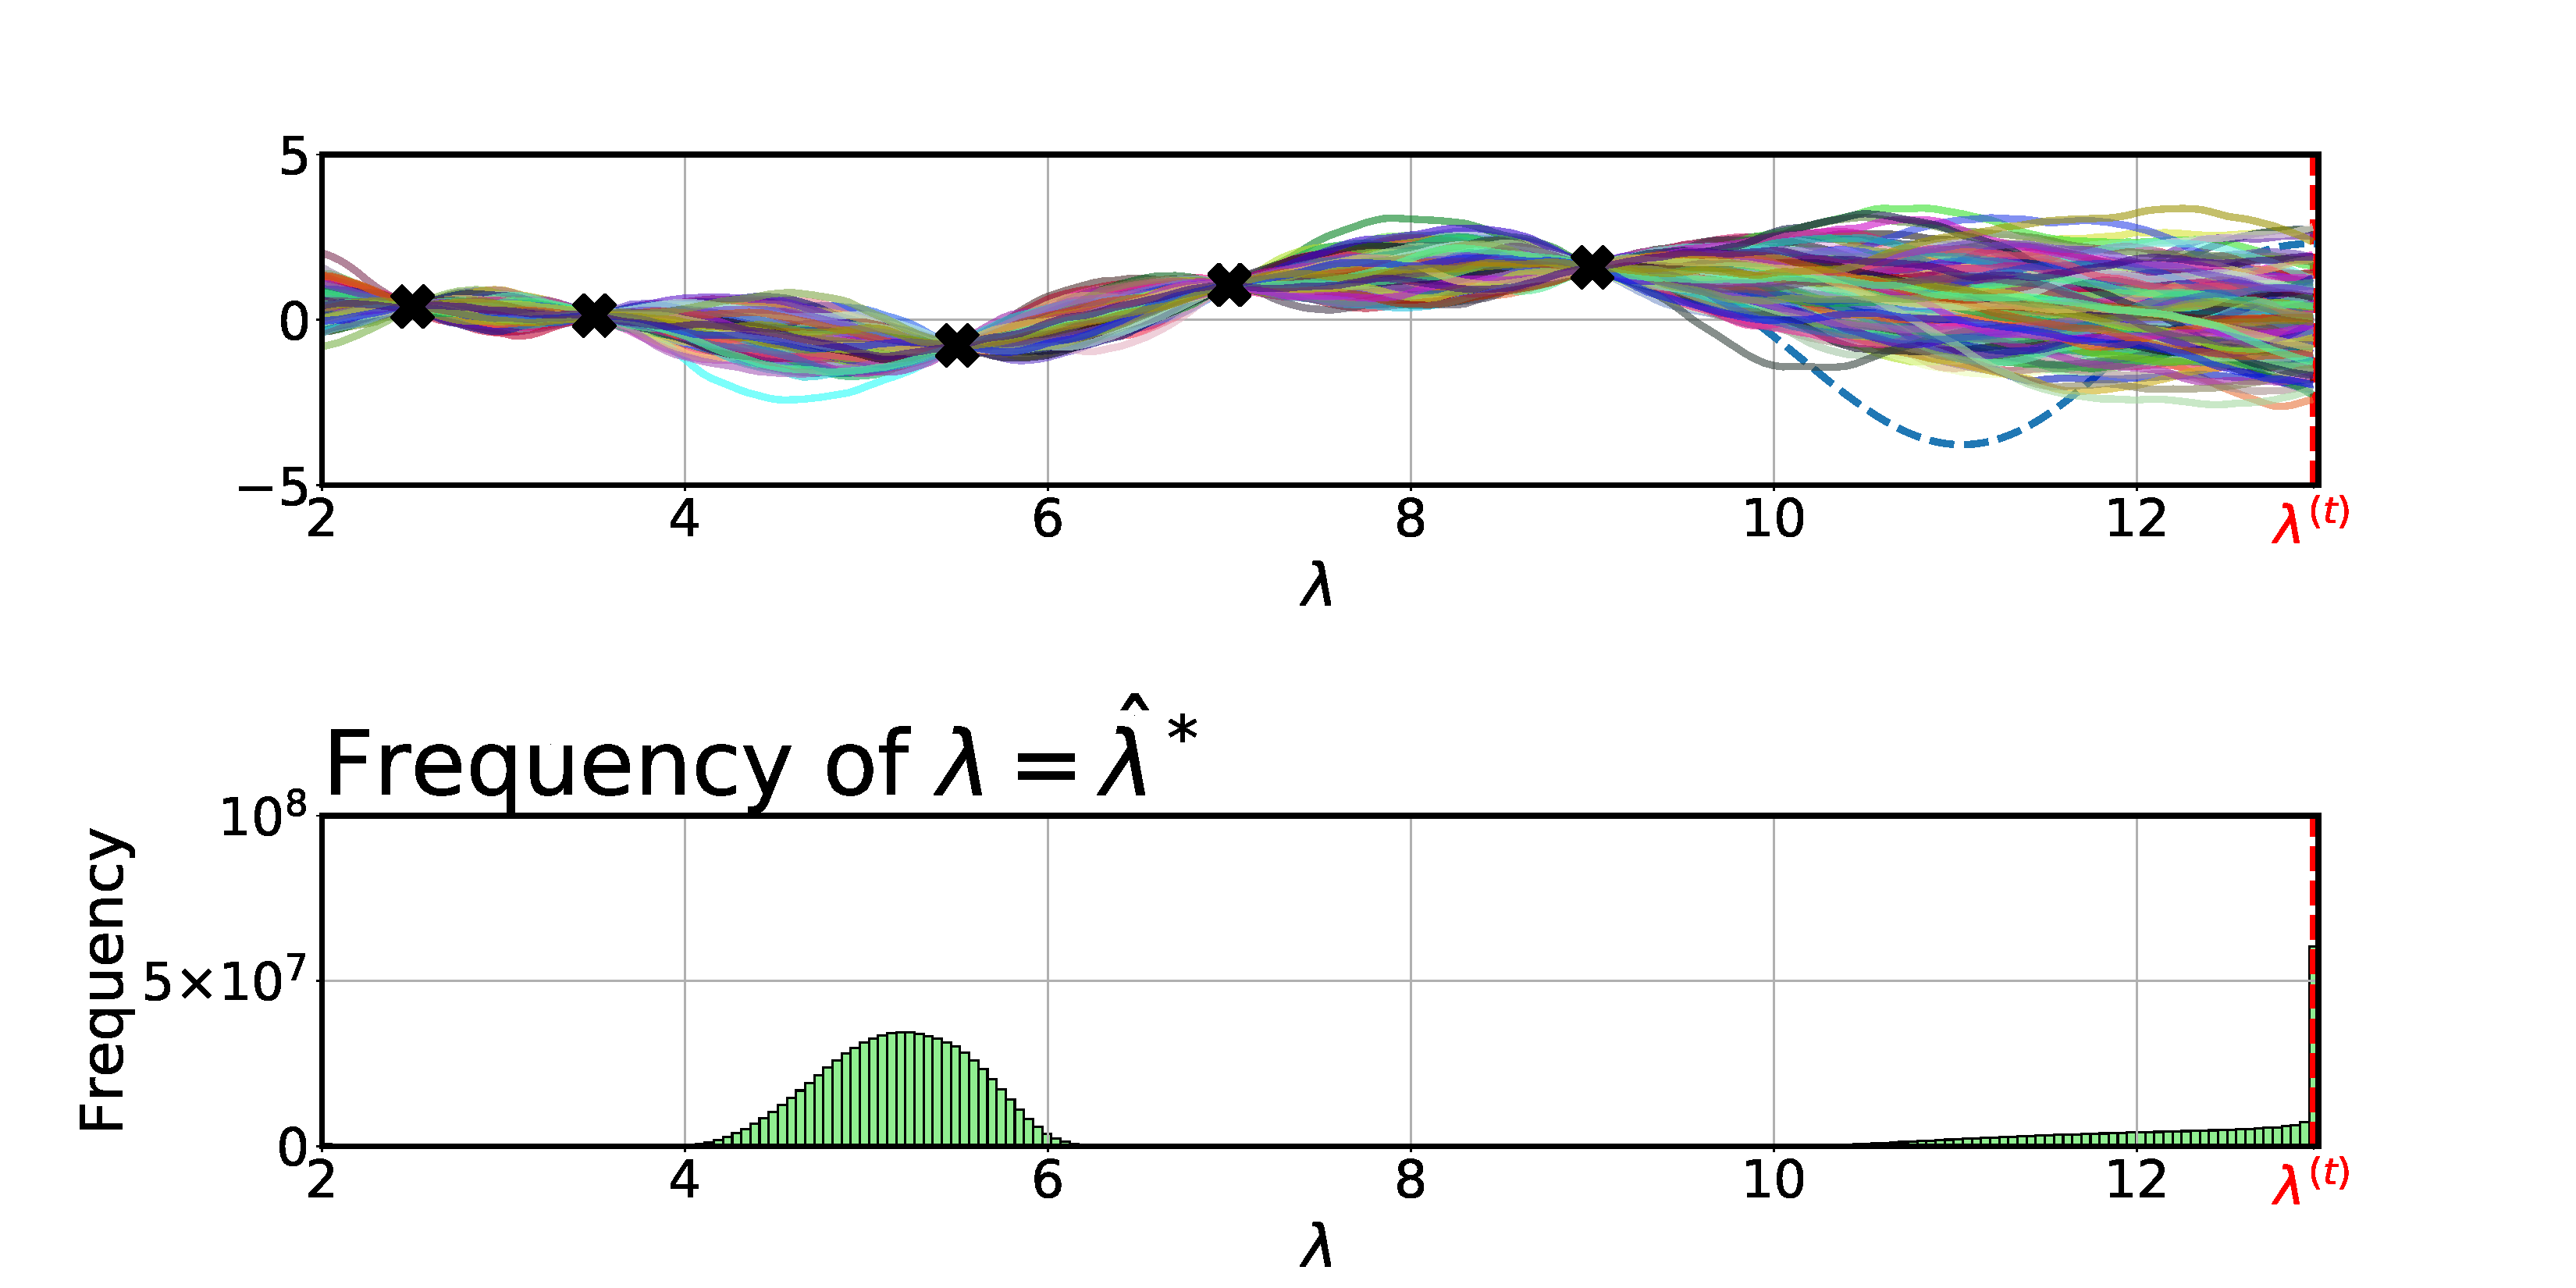
\includegraphics[width=\linewidth, height=0.7\textheight, keepaspectratio=true]{images/acq_func_images/es/es_6.pdf}};
    \node<.> [below=-1.0\belowcaptionskip of img6, align=center]{The configuration that is most likely to be $\conf^*$ provides the greatest information gain,\\ or in other words, would reduce the entropy of the search space the most when evaluated.};
  \end{tikzpicture}
\end{figure}

\end{frame}
% %----------------------------------------------------------------------
% \begin{frame}[c]{Computationally Expensive Acquisition Functions - ES}
% \framesubtitle{Entropy Search - Pseudocode for Sampling Version}

% \begin{center}
% \begin{minipage}{0.75\textwidth}
% \comment{Fix algorithm numbering}
% \begin{algorithm}[H]
%     %\DontPrintSemicolon
%     \LinesNumbered
%     \SetAlgoLined
%     \setcounter{AlgoLine}{0}
%     \SetKwInOut{Require}{Require}
%     \SetKwInOut{Result}{Result}
    
%     \Require{GP $\iter{\gp}$, budget $S$}
%     \Result{$\bonextsample$}
    
%     $E\leftarrow{\langle E_{\conf} = 0 \rangle}_{\conf\in\pcs}$\;
    
%     \For{$s=1$ \KwTo $S$}{
    
%         Sample $g_s\sim\iter{\gp}$\;
        
%         $\conf_s\leftarrow\argmin(g_s)$\;
        
%         $E[\conf_s]\leftarrow E[\conf_s] + 1$\;\tcp{Update Histogram count}}

%     $\acq\leftarrow\mathcal{\hat{P}}(E)$\tcp*{Generate PDF from histogram $E$}\;
%     $\bonextsample\leftarrow\argmax_{\conf\in\pcs}u(\conf)$\;

%     \caption{Sampling Based Entropy Search}
% \end{algorithm}
% \end{minipage}
% \end{center}

% \end{frame}
%-----------------------------------------------------------------------
\begin{frame}[c]{Computationally Expensive Acquisition Functions - ES}
\framesubtitle{Entropy Search - Pseudocode for Sampling Version}

\begin{center}
\begin{minipage}{0.75\textwidth}
\comment{Fix algorithm numbering}
\begin{algorithm}[H]
    %\DontPrintSemicolon
    \LinesNumbered
    \SetAlgoLined
    \setcounter{AlgoLine}{0}
    \SetKwInOut{Require}{Require}
    \SetKwInOut{Result}{Result}
    
    \Require{Gaussian process $\gp$, candidate configuration $\conf$, finite set of representer points $\pcs_{repr}$, dataset $\dataset$}
    \Result{Utility $\acq(\conf)$}
    
    $F\leftarrow{\langle F_{\conf} = 0 \rangle}_{\conf'\in\pcs_{repr}}$ - Frequencies to compute $p_{min}$\;
    
    \For{$s=1$ \KwTo $S$}{
    
        %Sample $\tilde{c}_s \sim \normaldist(\conf | \mu_{\iter{\gp}}, \sigma_{\iter{\gp}})$\;
        Sample $\tilde{c}_s \sim \gp$ at $\conf$\;
        
        $\gp_s \leftarrow{}$ Condition $\gp$ on $\dataset \cup \{\left\langle\conf, \tilde{c}_s\right\rangle\}$\;
        
        $\conf_s\leftarrow\argmin_{\conf' \in \conf_{cand}}(\gp_s)$\;
        
        $F[\conf_s]\leftarrow F[\conf_s] + 1$\;}

    $p_{min}(\conf') \leftarrow F_{\conf'} / \sum_{\conf'' \in \pcs_{repr}} F_{\conf''} \forall{\conf' \in \pcs_{repr}} $ \;
    
    $\acq\leftarrow\mathcal{H}(p_{min}) = - \sum_{\conf' \in \pcs_{repr}} p_{min}(\conf') \log p_{min}(\conf')$\;

    \caption{Sampling Based Entropy Search Acquisition Function}
\end{algorithm}
\end{minipage}
\end{center}

\end{frame}
%----------------------------------------------------------------------
\begin{frame}[c]{Computationally Expensive Acquisition Functions - ES}
\framesubtitle{Entropy Search - Varieties}
\begin{itemize}
    %\item<+-> Note how repeated Thompson Sampling inherently approximates sampling based entropy-search!
    \item<+-> A faster, but mathematically more involved version can be found in the \emph{original paper} on Entropy Search. \lit{\href{http://jmlr.csail.mit.edu/papers/volume13/hennig12a/hennig12a.pdf}{Hennig et al. 2012}}.
    \item<+-> Instead of computing ES directly, an alternative formulation called \emph{Predictive Entropy Search} is often used. \lit{\href{http://papers.nips.cc/paper/5324-predictive-entropy-search-for-efficient-global-optimization-of-black-box-functions.pdf}{Hernández-Lobato et al. 2014}}
    \item<+-> There exists a variant called \emph{Max-Value Entropy Search} which is cheaper to compute and has similar behavior. \lit{\href{https://arxiv.org/abs/1703.01968}{Wang and Jegelka 2017}}
    \item<+-> Further reading and summary for ES: \lit{\href{https://arxiv.org/pdf/1602.01064.pdf}{Metzen 2016}}.
\end{itemize}
\end{frame}
%-----------------------------------------------------------------------
\begin{frame}[c]{Questions to Answer for Yourself / Discuss with Friends}
\begin{itemize}
    %KG
    \item \emph{Repetition.} Describe the differences between KG and EI?
    %ES
    \item \emph{Discussion.} Is there an incentive for Entropy search to sample at $\max(p_{min})$? 
    \item \emph{Discussion.} How would you optimize the acquisition function in practice?
\end{itemize}
\end{frame}